\documentclass[11pt]{article}
\PassOptionsToPackage{dvipsnames}{xcolor}
\usepackage[review]{acl}

\usepackage[utf8]{inputenc}
\usepackage{latexsym}
\usepackage{microtype}
\usepackage{inconsolata}
\usepackage{hyperref}
\usepackage{url}
\usepackage{graphicx}
\usepackage{booktabs}
\usepackage{multirow}
\usepackage{amsmath}
\usepackage{amsfonts}
\usepackage{amssymb}
\usepackage{amsthm}
\usepackage{dsfont}
\usepackage{algorithm}
\let\AND\relax
\usepackage{algorithmic}
\usepackage[ruled,noend,algo2e]{algorithm2e}
\usepackage{tcolorbox}
\usepackage{subcaption}
\usepackage{enumitem}
\usepackage{array, rotating}
\usepackage{pifont}
\tcbuselibrary{skins,breakable}
\usepackage{adjustbox}
\usepackage{tabularx,makecell}
\usepackage{xspace}
% pgfplots figure pre-compiled as topology_scatter.pdf
\usepackage{xcolor}

% ACL 2026 submission
\newtheorem{theorem}{Theorem}
\newtheorem{assumption}{Assumption}

\newtcolorbox{examplebox}[1][]{
  colback=gray!5,
  colframe=gray!50,
  fonttitle=\bfseries,
  breakable,
  #1
}

\title{When Should Language Models Search? A Topology-Aware Analysis of Reasoning Strategies}
\author{Anonymous Author(s)}

\begin{document}
\maketitle

% \begin{abstract}
% Chain-of-thought (CoT) prompting is the default way to elicit reasoning from large language models, but it commits to a single linear trajectory and is therefore brittle on problems that require backtracking, multi-hop synthesis, or the comparison of competing hypotheses. We study a complementary alternative: a budgeted A*-style search over reasoning steps, where an LLM proposes successor steps and a conservative heuristic prioritizes which partial traces to expand. Across StrategyQA (2{,}290 examples), LogicQA (651 examples), and HotpotQA (500 examples), we find substantial instance-level complementarity between CoT and A*: the oracle that selects the correct strategy per instance reaches 84.59\%, 59.29\%, and 94.20\%, well above the best single-method, which yields 74.80\%, 45.78\%, and 80.10\%, respectively. We then evaluate routing strategies based on semantic entropy, a feature-based random forest, and an LLM-as-critic. Routing improves performance, but only partially closes the oracle gap: the best observed routers reach 76.25\% on StrategyQA, 48.20\% on LogicQA, and 81.30\% on HotpotQA. We complement the quantitative results with a diagnostic analysis showing that A* helps most on non-linear evidence aggregation, hypothesis elimination, and multi-hop chaining, whereas CoT remains preferable for direct factual recall and fluent world-knowledge integration. Our results suggest that the main opportunity is not replacing CoT with search, but learning when to deploy each reasoning strategy. Code is available at: \url{https://anonymous.4open.science/r/astar-reasoning-EC39}
% \end{abstract}


% \begin{abstract}
% Chain-of-thought (CoT) prompting generates a single reasoning trajectory, while search-based methods like A* explore multiple partial traces before committing. Which approach should an LLM use for a given problem? We find that neither dominates: across StrategyQA, LogicQA, HotpotQA, GSM8K, and MATH, CoT and A* each solve substantial instance subsets that the other misses. To explain this complementarity, we develop a \emph{Reasoning Topology Framework} built on 13 structural features computable from the input alone. A* advantage turns out to track a single derived quantity---branching coefficient---rather than dataset identity ($R^2=0.94$ across topology clusters). Building on this, we train a topology-aware router that sees no generated traces yet outperforms semantic-entropy and LLM-as-critic routers that inspect full reasoning chains, recovering 26.1\% of the oracle gap. We trace this counterintuitive result to a \emph{Fluency-Correctness Asymmetry}: in 38\% of disagreement cases the more fluent trace is actually wrong, systematically misleading post-hoc judges. Sensitivity sweeps, compute accounting, and 14B-scale experiments confirm that the topology-dependent pattern is robust. A* is not a universal upgrade over CoT; it is a higher-cost strategy best deployed when problem structure rewards branching. Code: \url{https://anonymous.4open.science/r/astar-reasoning-EC39}
% \end{abstract}



\begin{abstract}
Search-based reasoning and chain-of-thought (CoT) prompting offer two contrasting inference-time paradigms for language models: CoT commits to a single linear trajectory, while search explores alternative partial reasoning paths before selecting an answer. In this work, we study this trade-off using A* as a controlled and optimal instantiation of heuristic-guided search. Across eight benchmarks---StrategyQA, LogicQA, HotpotQA, GSM8K, MATH, HumanEval, MBPP, and CodeContests---and across three model scales, we find that search is not a universal upgrade over CoT; instead, the two strategies solve substantially different subsets of instances. To explain this complementarity, we introduce a \emph{Reasoning Topology Framework} based on structural features computable before generation. A derived \emph{branching coefficient} predicts when search helps better than dataset identity, indicating that the CoT--search boundary is primarily topology-dependent. We further train a topology-aware router that selects between CoT and A* without observing generated traces. Despite this restriction, it outperforms post-hoc routers based on semantic entropy and LLM-as-critic judgments. We attribute this to a \emph{Fluency--Correctness Asymmetry}: fluent traces are often incorrect, making trace-level adjudication unreliable. Overall, our results suggest that adaptive reasoning should route by problem structure, deploying search only when the input topology warrants its higher cost.
\end{abstract}




%=============================================================================
\section{Introduction}
\label{sec:intro}
%=============================================================================

Chain-of-thought (CoT) prompting~\cite{wei2022chain} has become the standard way to elicit step-by-step reasoning from large language models (LLMs). By generating intermediate reasoning steps before a final answer, CoT often improves performance on arithmetic, commonsense, and symbolic tasks. However, its core generation process is still strictly \emph{linear}: the model generates a single trace $s_1 \rightarrow s_2 \rightarrow \cdots \rightarrow s_T$, and later steps are conditioned on all earlier generated contents. This design creates three potential problems. First, an early mistake can propagate through the entire trace because the model has no built-in backtracking mechanism. Second, questions that require integrating several independent pieces of evidence can be difficult to solve with a single left-to-right narrative. Third, CoT has no explicit search objective that trades off trace length and alternative hypotheses.

These limitations motivate search-based reasoning. If the model can explore multiple partial traces, then it can reconsider early commitments, compare candidate branches, and prioritize promising reasoning states. In this paper, we study a budgeted A*-search procedure over natural-language reasoning traces. The language model generates successor steps, a step cost penalizes both trace length and low-confidence steps, and a heuristic prioritizes which partial trace to expand next.

But search is not free of problems. Exploring multiple branches can also waste computation on dead-end decompositions or introduce noise on problems that a single well-chosen chain would solve directly. In our experiments, we find that A* occasionally \emph{hurts} by overthinking simple questions (Section~\ref{sec:sensitivity}). The central question is therefore not ``is search better?'' but rather: \emph{which structural properties of a reasoning problem predict whether branching will help?}

Concretely, we ask the following research questions: (i)~Does guided search dominate CoT, or do they trade wins? (ii)~When they disagree, is the split random or systematic? (iii)~Can we predict which method will win from structural features of the input alone---before generating any reasoning trace from either CoT or the search procedure? (iv)~Does such a pre-generation router actually outperform post-hoc adjudication (such as an LLM based judge) that sees full reasoning traces?




% \paragraph{Motivating example.}
% Consider the StrategyQA question: \emph{``Is shrimp scampi definitely free of plastic?''} (gold answer: \textsc{No}). The CoT trace generated by LLaMA-3.1-8B proceeds through a five-step linear analysis of harvesting, processing, cooking, ingredient sourcing, and regulatory oversight. Each step is locally plausible, but the trace never surfaces the key fact that seafood can contain microplastics. The final answer is, therefore, wrong. In contrast, the A* trace reaches the biological premise almost immediately and then reasons that cooking does not remove microplastics, yielding the correct answer. The difference is not simply that one model ``knew more facts.'' It is that the search procedure prioritized a more relevant branch of the reasoning space.

\textbf{Motivating example.} On StrategyQA, linear CoT can pursue a locally plausible but ultimately irrelevant chain, while A* can surface the decisive evidence earlier by exploring alternative partial traces. For example (\S Figure \ref{fig:motivating_example}), on the question ``Is shrimp scampi definitely free of plastic?'', CoT misses the key fact of microplastic accumulation in seafood, whereas A* reaches that premise early and answers correctly. This illustrates the central hypothesis of the paper: CoT and search are complementary, and the real challenge is deciding when to use which. This pattern persists at scale. Across all benchmarks, CoT and A* solve different subsets of examples. On StrategyQA, A* outperforms CoT (74.80\% vs.\ 64.52\%), yet the oracle reaches 84.59\%. On LogicQA, CoT is slightly stronger (45.78\% vs.\ 44.85\%), but the oracle still reaches 59.29\%. Together, these gaps show that the main opportunity is \emph{strategy selection}: different questions favor different reasoning strategies.


% This pattern repeats at scale. Across our three evaluation benchmarks, CoT and A* succeed on systematically different subsets of examples. On StrategyQA, A* outperforms CoT (74.80\% vs.\ 64.52\%), but the oracle that selects the correct method per instance reaches 84.59\%, leaving a 9.79-point gap above the better single method. On LogicQA, CoT is slightly better than A* (45.78\% vs.\ 44.85\%), yet the oracle still reaches 59.29\%, a 13.51-point gap. On HotpotQA, A* again leads CoT (80.10\% vs.\ 76.80\%), while the oracle reaches 94.20\%, a further 14.10-point gap. These numbers suggest that the real opportunity lies in \emph{strategy selection}: different questions appear to favor different reasoning algorithms.


% On HotpotQA, A* again leads (80.10\% vs.\ 76.80\%), while the oracle reaches 94.20\%. 


\paragraph{Why A* specifically?}
Our goal is not to champion A* as the best search algorithm for LLMs, but to use it as a controlled diagnostic. A* separates the key ingredients of guided search---a priority frontier, a path cost, and a heuristic estimate---without entangling them with evaluator design (as in ToT), rollout policies (as in MCTS), or fixed-width pruning (as in beam search). This makes it easier to isolate \emph{when} the act of branching itself is responsible for gains.

\paragraph{Contributions.}
Our contributions: (1)~We compare CoT and A* across eight benchmarks spanning QA, math, and code generation (StrategyQA, LogicQA, HotpotQA, GSM8K, MATH, HumanEval, MBPP, CodeContests) and three model scales (0.5B, 8B, 14B), finding that neither uniformly dominates. (2)~We quantify instance-level complementarity: CoT and A* solve genuinely different subsets, and the oracle gap is large enough to make routing worthwhile. (3)~We introduce 13 pre-generation topology features and show that a single derived quantity---branching coefficient---predicts A* advantage better than dataset identity ($R^2=0.94$). (4)~We show that a topology-aware router outperforms post-hoc trace evaluation, and diagnose why through a Fluency-Correctness Asymmetry analysis.









\begin{figure}[t]
\centering
\begin{tcolorbox}[
    enhanced,
    colback=white,
    colframe=black!75,
    boxrule=0.7pt,
    arc=1.8mm,
    left=6pt, right=6pt, top=6pt, bottom=6pt,
    title=\textbf{Motivating Example}\hfill
    \emph{Query: ``Is shrimp scampi definitely free of plastic?''}\hfill
    \textbf{Gold: \textsc{False}},
    colbacktitle=black!4,
    coltitle=black,
    fonttitle=\small
]
\footnotesize

\begin{minipage}[t]{0.485\textwidth}
\begin{tcolorbox}[
    enhanced,
    colback=red!2,
    colframe=red!65!black,
    boxrule=0.5pt,
    arc=1.2mm,
    left=5pt, right=5pt, top=4pt, bottom=4pt,
    title=\textbf{\color{red!75!black}\ding{55} Chain-of-Thought}\hfill \emph{Linear generation},
    colbacktitle=red!6,
    coltitle=black,
    fonttitle=\footnotesize
]
\textit{Commits to a chronological schema, missing the biological premise.}

\vspace{2pt}
\begin{itemize}
    \setlength{\itemsep}{1pt}
    \setlength{\parskip}{0pt}
    \item[\textbf{S1.}] Shrimp are caught/farmed; no conclusive evidence of significant plastic.
    \item[\textbf{S2.}] Processing does not involve contamination.
    \item[\textbf{S3.}] Cooking does not introduce plastic.
    \item[\textbf{S4.}] No evidence of ingredient contamination.
    \item[\textbf{S5.}] Regulatory standards make contamination unlikely.
    \item[\textbf{Ans.}] \textsc{Yes} \hfill \textbf{(Incorrect)}
\end{itemize}
\end{tcolorbox}
\end{minipage}
\hfill
\begin{minipage}[t]{0.485\textwidth}
\begin{tcolorbox}[
    enhanced,
    colback=blue!2,
    colframe=blue!65!black,
    boxrule=0.5pt,
    arc=1.2mm,
    left=5pt, right=5pt, top=4pt, bottom=4pt,
    title=\textbf{\color{blue!75!black}\ding{51} A* Search}\hfill \emph{Heuristic-guided},
    colbacktitle=blue!6,
    coltitle=black,
    fonttitle=\footnotesize
]
\textit{Prioritizes the key biological premise directly.}

\vspace{2pt}
\begin{itemize}
    \setlength{\itemsep}{1pt}
    \setlength{\parskip}{0pt}
    \item[\textbf{S1.}] Shrimp often contain microplastics in tissues.
    \item[\textbf{S2.}] Preparation does not remove pre-existing microplastics.
    \item[\textbf{Ans.}] \textsc{False} \hfill \textbf{(Correct)}
\end{itemize}
\end{tcolorbox}
\end{minipage}

\end{tcolorbox}

\vspace{-2mm}
\caption{Comparison of reasoning trajectories on a StrategyQA example. CoT follows a plausible but misdirected chronological schema, while A* prioritizes the key biological fact—microplastic presence in shrimp—and reaches the correct conclusion with fewer, more relevant steps.}
\label{fig:motivating_example}
\end{figure}


% \medskip

%=============================================================================
\section{Methodology}
\label{sec:method}
%=============================================================================

We first formalize CoT and search-based reasoning under a common notation and then describe the routing mechanisms that choose between them.

%-----------------------------------------------------------------------------
\subsection{Notation and Problem Setup}
\label{sec:notation}
%-----------------------------------------------------------------------------

Let $\mathcal{Q} = (q, C, \mathcal{O})$ denote a reasoning problem, where $q$ is the question, $C$ is an optional context passage, and $\mathcal{O} = \{o_1, \ldots, o_K\}$ is the candidate answer set for multiple-choice tasks or the output space for free-form tasks. A \emph{reasoning trace} $\tau = (s_1, s_2, \ldots, s_T)$ is an ordered sequence of natural-language reasoning steps, and a prediction function $\phi(\tau) \in \mathcal{O}$ extracts the final answer from the trace. Let $\mathcal{M}_\theta$ denote a language model with parameters $\theta$.

%-----------------------------------------------------------------------------
\subsection{Chain-of-Thought (CoT) Reasoning}
\label{sec:cot}
%-----------------------------------------------------------------------------

In CoT prompting, the model generates a single reasoning trace autoregressively: $\tau^{\text{CoT}} = (s_1, s_2, \ldots, s_T)$ and $s_t \sim \mathcal{M}_\theta(\cdot \mid q, C, \mathcal{O}, s_{1:t-1})$.
Generation terminates when the model emits a terminal answer pattern, and the final prediction is $\hat{y}^{\text{CoT}} = \phi(\tau^{\text{CoT}})$. CoT explores exactly one element of the trace space with no mechanism for backtracking or branch comparison.

%-----------------------------------------------------------------------------
\subsection{A* Search over Reasoning Traces}
\label{sec:astar}
%-----------------------------------------------------------------------------

We therefore search over the space of reasoning traces using an A*-style priority rule, but with a finite node budget and a multi-goal voting procedure for tractability.

\paragraph{State space.}
The search space is a tree $\mathcal{G} = (\mathcal{S}, \mathcal{E})$ where each node $n \in \mathcal{S}$ represents a partial reasoning state: $n = (\tau_n, d_n), \qquad \tau_n = (s_1, \ldots, s_{d_n})$. Here, $\tau_n$ is the partial trace stored at node $n$ and $d_n = |\tau_n|$ is its depth. The root node $n_0$ has $\tau_{n_0} = \emptyset$ and $d_{n_0} = 0$. An edge $(n,n') \in \mathcal{E}$ exists when $\tau_{n'} = \tau_n \oplus s$ for some reasoning step $s$.

\paragraph{Successor generation.}
Given a node $n$ with state $(\tau_n, d_n)$, we ask the language model to propose $N_c$ candidate next steps:
\begin{equation}
\{(s^{(j)}, c^{(j)})\}_{j=1}^{N_c} = \textsc{GS}(\mathcal{M}_\theta, q, C, \mathcal{O}, \tau_n, N_c).
\label{eq:successor}
\end{equation}
\textsc{GS} refers to the step-generation function. Each candidate consists of step text $s^{(j)}$ and a self-reported confidence $c^{(j)} \in [0.0,1.0]$. The candidate induces a successor node $n'_j$ with trace $\tau_{n'_j} = \tau_n \oplus s^{(j)}$ and depth $d_{n'_j} = d_n + 1$.

\paragraph{Goal condition.}
A node is a goal node if its last step contains a terminal answer pattern:
\begin{equation}
\textsc{IsGoal}(n) = \mathds{1}\Big[\exists p \in \mathcal{P}: p \subset s_{d_n}\Big],
\label{eq:isgoal}
\end{equation}
where $\mathcal{P}$ contains answer templates such as ``The answer is [A/B/C/D]'' for multiple-choice tasks.

\paragraph{Path cost.}
The cumulative cost of a node trades off reasoning length and uncertainty:
\begin{equation}
g(n) = \sum_{t=1}^{d_n} \big[1 + (1-c_t)\big]
    = d_n + \sum_{t=1}^{d_n}(1-c_t).
\label{eq:gcost}
\end{equation}
\textit{Each step contributes a base cost of 1, and lower-confidence steps incur an additional penalty. This makes shorter, higher-confidence traces cheaper than longer or more uncertain ones.}

% \subsection{Heuristic Design and Admissibility Guarantee}
% \label{sec:heuristic_design}


% % For LogicQA, the implementation uses a related remaining-depth and logical-complexity heuristic. This reflects the fact that LogicQA instances often require comparing compact argument structures rather than accumulating entity coverage. We therefore treat LogicQA's heuristic as an implementation-specific variant and do not claim that the theorem below applies to that variant. The theorem applies to the depth-plus-coverage heuristic used for StrategyQA and HotpotQA.


% \paragraph{Assumption 1: Minimum-hop lower bound.}
% Any valid goal trace requires at least \(H_{\min}\) reasoning steps from the root. Equivalently, for any non-goal node with depth \(d_n < H_{\min}\), at least \(H_{\min}-d_n\) further transitions are required before reaching a goal.

% \paragraph{Assumption 2: Non-goal continuation.}
% Any non-goal node with depth \(d_n \geq H_{\min}\) still requires at least one additional transition before reaching a goal.

% \paragraph{Theorem 1: Conservative admissibility.}
% Under Assumptions 1 and 2, if

% $\omega_d+\omega_c \leq c_{\min}$, then the depth-plus-coverage heuristic is admissible for all non-goal nodes; that is, $h(n) \leq h^*(n)$, where $h^*(n)$ is the true minimum remaining path cost from node \(n\) to a valid goal.

% \paragraph{Proof.}

% Formal proof is there in Section \ref{full-proof}.


\subsection{Heuristic Design and Admissibility Guarantee}
\label{sec:heuristic_design}

The heuristic estimates the remaining cost from a partial trace to a valid goal. In our implemented A* system, we use lightweight, interpretable search-control signals rather than a learned verifier. Across datasets, the heuristic combines depth and coverage: $h(n)=h_{\mathrm{depth}}(n)+h_{\mathrm{coverage}}(n)$ with
\begin{multline}
h_{\mathrm{depth}}(n)=\omega_d\max(0,H_{\min}-d_n),
\\
h_{\mathrm{coverage}}(n)=\omega_c(1-E(n)).
\end{multline}
Here \(H_{\min}\) is a task-level lower bound on required reasoning hops from the root, \(d_n\) is the depth of node \(n\), \(E(n)\in[0,1]\) is the fraction of target entities or constraints already covered by the partial trace, and \(\omega_d,\omega_c>0\) are heuristic weights. Thus, \(h_{\mathrm{depth}}\) encourages search to continue until a minimum reasoning depth is reached, while \(h_{\mathrm{coverage}}\) favors traces that cover more answer-relevant entities or constraints. Let $c_{\min}=1+(1-c_{\max})$ be the minimum possible transition cost under the path-cost definition. Since each transition has base cost \(1\) plus uncertainty penalty \(1-c_t\), every transition costs at least \(c_{\min}\). The confidence and coverage terms are practical search-control signals, not calibrated uncertainty estimates or exact measures of evidential completeness.

\paragraph{Assumption 1: Minimum-hop lower bound.}
Any valid goal trace requires at least \(H_{\min}\) reasoning steps from the root; equivalently, any non-goal node with \(d_n < H_{\min}\) requires at least \(H_{\min}-d_n\) further transitions.

\paragraph{Assumption 2: Non-goal continuation.}
Any non-goal node with \(d_n\geq H_{\min}\) still requires at least one additional transition before reaching a goal.

\paragraph{Theorem 1: Conservative admissibility.}
Under Assumptions 1 and 2, if \(\omega_d+\omega_c\leq c_{\min}\), then the depth-plus-coverage heuristic is admissible for all non-goal nodes:
\[
h(n)\leq h^*(n),
\]
where \(h^*(n)\) is the true minimum remaining path cost from node \(n\) to a valid goal.

\paragraph{Proof.}
The formal proof is provided in Section~\ref{full-proof}.




\paragraph{Operational instantiation: a symbolic progress scorer.}
The abstract heuristic in Eq.~(6)--(8) is instantiated as a
dataset-agnostic progress estimator over partial reasoning states. Unlike
a learned verifier or LLM-based critic, this estimator does not judge the
truth of a partial trace directly. Instead, it plays a critic-like
search-control role by assigning lower remaining cost to states that have
made sufficient structural progress: reaching the minimum reasoning depth
and covering question-relevant entities. For a question \(q\), we extract
a set of content units \(\mathcal{E}_q\) consisting of quoted strings,
proper-name phrases, numbers, years, and non-stopword content terms. For
a node \(n\) with partial trace \(\tau_n\), coverage is computed as
\[
E(n)=
\frac{|\{e\in\mathcal{E}_q: e \text{ appears in } \tau_n\}|}
{|\mathcal{E}_q|},
\]
with \(E(n)=1\) when no content units are extracted. The implemented
heuristic is
\[
h(n)
=
\omega_d\max(0,H_{\min}-d_n)
+
\omega_c(1-E(n)).
\]
Thus, the heuristic is an operational instantiation of the
depth--coverage template: \(h_{\mathrm{depth}}\) estimates remaining
structural progress, while \(h_{\mathrm{coverage}}\) estimates remaining
content coverage. Because the same extraction and scoring rule is applied
across datasets, the heuristic is dataset-agnostic even though its
minimum-hop parameter can encode a task-level lower bound. In Appendix Section \ref{more-on}, it is described why this is dataset agnostic (with an example) and we report a human analysis which shows this critic based heuristics underestimates human-assessed progress.




%-----------------------------------------------------------------------------

%-----------------------------------------------------------------------------
\subsection{Routing Strategies}
\label{sec:routing}
%-----------------------------------------------------------------------------

Given the complementarity between CoT and A*, we define routing functions $\mathcal{R}: \mathcal{Q} \to \{\text{CoT}, A^*\}$. We distinguish two families.

\paragraph{Output-based routers.} They require generating traces before deciding. \emph{Semantic entropy}~\citep{kossen2024semanticentropyprobesrobust}: routes high-entropy (under self-consistency) instances to A*. \emph{LLM-as-critic}: on disagreements, a critic model (DeepSeek-R1-Distill-Qwen-14B, chosen for architectural distinctness from the LLaMA-3.1-8B backbone and local executability) compares both traces:
\begin{equation}
\text{verdict} = \mathcal{M}_{\text{critic}}(\text{Trace}_{\text{CoT}}, \text{Trace}_{A^*}, q, C, \mathcal{O})
\label{eq:critic}
\end{equation}

\paragraph{Pre-generation routers.} They decide before any generation. \emph{Random forest}: trained on hand-crafted features (question length, connectives, negation). \emph{Topology router} (hereafter \emph{CoT--A* router}): XGBoost on the 13 topology features, requiring no LLM inference at routing time. It is a diagnostic test of whether the CoT/A* boundary is predictable from problem structure.

\paragraph{Terminology clarification.} We distinguish three uses of evaluation/scoring in this work:
\begin{itemize}[nosep,leftmargin=*]
\item \emph{Rule-based progress scorer}: the deterministic heuristic $h(n)$ used to prioritize partial states during A* search (Eq.~\ref{eq:heuristic}). Not an LLM.
\item \emph{LLM-as-Critic}: an output-based router that inspects both completed CoT and A* traces and selects between them via pairwise comparison.
\item \emph{LLM-as-Judge}: an alternative output-based router using a different prompting formulation emphasizing faithfulness and logical validity.
\end{itemize}


\subsection{Reasoning Topology Features based Routing}
\label{sec:topology_features}
%-----------------------------------------------------------------------------

% To characterize the structural demands of a reasoning problem \emph{before} any model generation, we define 13 pre-generation features computed directly from the input text: question length, context length, context sentences, logical connectives, negation markers, comparatives, question marks, estimated hop count (dependency-based), contextual density (entities/sentence), distractors, reasoning depth, number of options, and a key derived feature---the \emph{branching coefficient} $\text{bc} = \text{c\_sent} \times \text{hop} / \text{q\_len}$---which captures how much branching structure the input affords. These features require no model inference and are used for both topology clustering (\S\ref{sec:topology_clusters}) and pre-generation routing (\S\ref{sec:topology_routing}).


To characterize the structural demands of a reasoning problem \emph{before} any model generation, we define 13 pre-generation features computed directly from the input text. These include surface length features---question length, context length, and number of context sentences; syntactic and discourse cues---logical connectives, negation markers, comparatives, and question marks; reasoning-structure features---estimated hop count from dependency links, contextual density measured as entities per sentence, distractor count, and estimated reasoning depth; and task-format features such as the number of answer options. We also define a derived \emph{branching coefficient}:
\begin{equation}
\mathrm{BC} = \frac{\mathrm{c\_sent} \times \mathrm{hop}}{\mathrm{q\_len}}
\label{eq:branching_coefficient}
\end{equation}
where $\mathrm{c\_sent}$ is the number of context sentences, $\mathrm{hop}$ is the estimated reasoning-hop count, and $\mathrm{q\_len}$ is the question length. BC summarizes how much multi-hop branching structure the input affords relative to question length.
These features require no model inference and are used for both topology clustering (\S\ref{sec:topology_clusters}) and pre-generation routing (\S\ref{sec:topology_routing}).

\paragraph{Router evaluation protocol.} The topology-aware router (referred to as the \emph{CoT--A* router}) is evaluated using stratified 5-fold cross-validation (seed 42), performed separately within each benchmark. For each fold, the router is trained on four folds and evaluated only on the held-out fold; no evaluation instance is used to train the router that predicts it. The router receives only the 13 pre-generation features---it does not observe CoT traces, A* traces, model confidence, predicted answers, or gold answers at inference time. This protocol evaluates \emph{within-dataset generalization}; cross-dataset transfer is examined separately via a leave-one-benchmark-out experiment (Appendix~\ref{app:leave_one_out}).




%=============================================================================
\section{Results}
\label{sec:results}
%=============================================================================

We evaluate on eight benchmarks using three models: i) LLaMA-3.1-8B, ii) Qwen-0.5B, and iii) Qwen-2.5-14B, and we use DeepSeek-R1-Distill-Qwen-14B as the LLM critic. For QA, we use StrategyQA~\cite{geva2021did} (multi-step commonsense, boolean answers), LogicQA~\cite{liu2020logiqa} (formal logical reasoning, four-way multiple choice), and HotpotQA~\cite{yang2018hotpotqa} (multi-hop QA, free-form answers). For math, we use GSM8K~\cite{cobbe2021trainingverifierssolvemath} and MATH~\cite{hendrycks2021measuringmathematicalproblemsolving}. For code generation, we use HumanEval~\cite{chen2021humaneval} (163 function-level tasks with detailed docstrings), MBPP~\cite{austin2021mbpp} (500 tasks with one-sentence specifications), and CodeContests~\cite{li2022codecontests} (500 algorithmic problems). We report exact accuracies from the current experimental pipeline, and the oracle corresponds to instance-wise selection of the correct answer between CoT and A*.

%-----------------------------------------------------------------------------
\subsection{Quantitative Analysis}
\label{sec:quantitative}
%-----------------------------------------------------------------------------


% Self-Consistency (LLaMA-3.1-8B) & 71.22\% & 46.10\% & 78.21\% \\

% Tree-of-Thought (LLaMA-3.1-8B) & 72.24\% & 46.21\% & 78.45\% \\





















\begin{table}[t]
\centering
\scriptsize
\setlength{\tabcolsep}{2.8pt}
\renewcommand{\arraystretch}{1.08}
\resizebox{0.75\textwidth}{!}{
\begin{tabular}{lcccc|cccc|cccc}
\toprule
\multirow{2}{*}{Dataset}
& \multicolumn{4}{c}{LLaMA-3.1-8B}
& \multicolumn{4}{c}{Qwen-0.5B}
& \multicolumn{4}{c}{Qwen-2.5-14B} \\
\cmidrule(lr){2-5}
\cmidrule(lr){6-9}
\cmidrule(lr){10-13}
& CoT & A* & SC & ToT
& CoT & A* & SC & ToT
& CoT & A* & SC & ToT \\
\midrule
StrategyQA
& 64.52 & \textbf{74.80} & 71.22 & \underline{72.24}
& \underline{53.60} & 53.40 & \textbf{54.21} & 52.24
& 76.02 & 75.56 & \textbf{80.06} & \underline{78.17} \\

LogicQA
& 45.78 & 44.85 & \underline{46.10} & \textbf{46.21}
& \textbf{24.00} & 20.20 & \underline{22.10} & 21.19
& \underline{57.91} & 58.12 & \textbf{59.19} & 55.12 \\

HotpotQA
& 76.80 & \textbf{80.10} & 78.21 & \underline{78.45}
& 8.40 & \textbf{30.00} & 12.21 & \underline{22.17}
& 60.19 & \textbf{83.33} & 65.25 & \underline{72.14} \\

GSM8K
& 85.04 & \underline{86.12} & \textbf{86.90} & 60.00
& \underline{26.84} & 14.48 & \textbf{43.22} & 41.02
& 61.56 & \textbf{80.59} & 50.57 & 48.82 \\

MATH
& 78.00 & \underline{79.10} & \textbf{79.50} & 40.10
& \textbf{32.80} & 16.20 & 41.60 & \textbf{49.00}
& 44.00 & \textbf{47.20} & 9.80 & 21.20 \\
\midrule
\multicolumn{13}{c}{\textit{Code Generation}} \\
\midrule
HumanEval
& \underline{67.48} & 64.42 & 65.03 & \textbf{71.78}
& \textbf{33.74} & 20.25 & 26.38 & \underline{33.13}
& 77.91 & 76.07 & \underline{76.07} & \textbf{79.75} \\

MBPP
& \textbf{39.80} & 36.80 & 38.00 & \underline{40.40}
& \textbf{24.00} & \underline{20.80} & 21.40 & 23.00
& 46.60 & 45.00 & \underline{46.80} & \textbf{49.80} \\

CodeContests
& 77.40 & \textbf{87.00} & \underline{99.00} & 91.20
& 49.80 & \textbf{68.20} & \underline{48.80} & 67.80
& \textbf{99.60} & 94.40 & \underline{98.20} & 94.00 \\
\bottomrule
\end{tabular}
}
\caption{Consolidated results across reasoning, math, and code generation benchmarks. Scores denote accuracy (\%). SC denotes Self-Consistency and ToT denotes Tree-of-Thought. Within each dataset--model block, the best single-method score is bolded and the second-highest is underlined. On CodeContests at 0.5B, A* gives a +18.4\,pp gain over CoT, mirroring the search advantage for small models on HotpotQA.}
\label{tab:consolidated-main-results}
\end{table}




\paragraph{Main results.}
Table~\ref{tab:consolidated-main-results} shows that no single reasoning strategy dominates across datasets, models, or reasoning formats. For LLaMA-3.1-8B, A* is substantially stronger than CoT on StrategyQA (+10.28\,pp) and HotpotQA (+3.30\,pp), while CoT has a slight edge on LogicQA (+0.93\,pp). Yet the oracle remains far above the better of CoT and A*---by +9.79, +13.51, and +14.10 points on StrategyQA, LogicQA, and HotpotQA, respectively---confirming strong instance-level complementarity. 
% The substantial CoT-only and A*-only cells in Table~\ref{tab:complementarity} further indicate that the methods implement genuinely different computations, motivating the topology analysis (Section~\ref{sec:topology_clusters}) and routing study (Section~\ref{sec:topology_routing}).

The expanded results show that this complementarity is not limited to one model or dataset family. On Qwen-0.5B, A* gives a large gain on HotpotQA (30.00 vs.\ 8.40), but not on StrategyQA or LogicQA, suggesting that search helps small models mainly when the task structure rewards exploration. On Qwen-2.5-14B, A* is especially effective on HotpotQA (83.33 vs.\ 60.19) and on GSM8K (80.6\% vs.\ 61.6\%, +19.0\,pp)---the largest A* advantage at any scale on math---while self-consistency is strongest on StrategyQA and LogicQA. Overall, search is most useful for multi-hop or branch-heavy inputs, whereas sampling-based or linear methods remain competitive on more compact reasoning problems. Finally, the best-router and oracle columns show that adaptive strategy selection can exceed any fixed single method, although a substantial oracle gap remains for the topology-aware routing.

The code-generation benchmarks show a similar trade-off. On CodeContests, A* outperforms CoT at both 0.5B (+18.4\,pp) and 8B (+9.6\,pp), with oracle gaps of 7.8\,pp and 9.2\,pp respectively---substantial complementarity that the topology router exploits effectively (95.0\% at 8B, recovering 87\% of the oracle gap). On HumanEval and MBPP, ToT is the strongest single method, but the oracle gap remains large (74.8\% at 8B, 85.9\% at 14B vs.\ best single). We present topology routing, multi-return analysis, and category breakdowns for code in Appendix~\ref{app:code_generation}.

% \paragraph{Router performance.}
% Routing closes only part of the oracle gap. The feature-based random forest reaches 76.25\% on StrategyQA (+1.45 over A*) and 48.20\% on LogicQA (+2.42 over CoT). These gains are real but much smaller than the oracle margin. The LLM-as-critic router runs only on the $\sim$25\% of disputed cases but gains are modest, suggesting that adjudicating between traces is difficult---especially when A* traces are less fluent yet logically stronger (analyzed further in Section~\ref{sec:topology_routing}).



\paragraph{Router performance.}
We evaluate all routing strategies on LLaMA-3.1-8B to test whether a router can choose between CoT and A* more effectively than either fixed strategy. Table~\ref{tab:topology_router} shows that routing closes only part of the oracle gap, but the topology-aware router is consistently strongest: on the QA benchmarks, it improves over the stronger fixed baseline by +2.55\,pp on StrategyQA, +3.23\,pp on LogicQA, and +2.31\,pp on HotpotQA, while recovering 26.1\% of the oracle gap. The pattern also extends to math, where the topology router reaches 91.10\% on GSM8K and 81.52\% on MATH, outperforming CoT, A*, semantic entropy, LLM-as-critic, LLM-as-judge, and random-forest routing. This contrast is important: trace-based routers yield only modest gains and sometimes underperform A* alone, whereas the topology router uses only 13 pre-generation structural features. Thus, the CoT--search decision is better predicted from problem topology than from retrospective evaluation of completed reasoning traces.


\begin{table}[ht]
\centering
\small
\adjustbox{width=\columnwidth}{\begin{tabular}{lcccc}
\toprule
\textbf{Dataset} & \textbf{Both correct} & \textbf{CoT only} & \textbf{A* only} & \textbf{Both wrong} \\
\midrule
StrategyQA  & 1361 (59.4\%) & 328 (14.3\%) & 248 (10.8\%) & 353 (15.4\%) \\
LogicQA       & 180 (27.6\%)  & 118 (18.1\%) & 88 (13.5\%)  & 265 (40.7\%) \\
HotpotQA     & 298 (59.6\%)  & 86 (17.2\%)  & 87 (17.4\%)  & 29 (5.8\%) \\
\midrule
HumanEval (8B) & 93 (57.1\%) & 17 (10.4\%) & 12 (7.4\%) & 41 (25.2\%) \\
MBPP (8B) & 163 (32.6\%) & 36 (7.2\%) & 21 (4.2\%) & 280 (56.0\%) \\
CodeContests (8B) & 341 (68.2\%) & 46 (9.2\%) & 94 (18.8\%) & 19 (3.8\%) \\
CodeContests (0.5B) & 210 (42.0\%) & 39 (7.8\%) & 131 (26.2\%) & 120 (24.0\%) \\
\bottomrule
\end{tabular}}
\caption{Instance-level complementarity decomposition. ``CoT only'' means CoT is correct and A* is wrong; ``A* only'' means the reverse.}
\label{tab:complementarity}
\end{table}

\paragraph{Instance-level decomposition.}
Table~\ref{tab:complementarity} makes the complementarity concrete. HotpotQA is especially striking: only 5.8\% of instances are missed by both strategies, while 34.6\% lie in a regime where exactly one strategy is correct. StrategyQA also exhibits sizable disagreement. LogicQA is harder overall, as shown by the 40.7\% ``both wrong'', but even there each strategy recovers failures of the other.



% We now group examples into diagnostic categories to explain \emph{why} the two strategies differ.

% \subsubsection{Patterns of A* Success and CoT Failure}
% \label{sec:astar_success}

% We identify three recurring settings where A* succeeds while CoT fails.

% \paragraph{Group 1: Non-linear evidence aggregation.}
% These are questions where the answer requires combining several facts that do not naturally form a single left-to-right narrative.



% \paragraph{Group 2: Hypothesis elimination.}
% A* is also effective when the problem naturally decomposes into evaluating or eliminating alternatives.


% \paragraph{Group 3: Multi-hop question answering.}
% HotpotQA highlights the value of search when the answer depends on chaining facts across sources.


% \subsubsection{Patterns of CoT Success and A* Failure}
% \label{sec:cot_success}

% We identify two common settings where CoT remains better than search.

% \paragraph{Group 1: Direct factual reasoning.}
% When the answer follows directly from familiar facts, search can introduce unnecessary branching and semantic drift.



% \paragraph{Group 2: Fluent world knowledge and argumentation.}
% When the problem is best solved by a smooth, coherent narrative, CoT often remains more reliable than fragmented search steps.


% \subsubsection{A* Failure Modes on Simple Cases}
% \label{sec:astar_failures}

% We observe three recurrent failure modes for A* on examples that CoT solves easily.

% \paragraph{Failure mode 1: Overthinking simple questions.}


% \paragraph{Failure mode 2: Spurious correlations in search.}


% \paragraph{Failure mode 3: Step repetition.}





% Manual inspection of disagreement cases reveals recurring regimes (detailed examples in Appendix~\ref{app:qualitative_examples}). \textbf{A* helps} when reasoning has branching structure: (i)~non-linear evidence aggregation, (ii)~hypothesis elimination, and (iii)~multi-hop composition---all cases where \emph{deferred commitment} is valuable. \textbf{CoT remains preferable} on single-path reasoning: direct factual recall and coherent argumentation where branching fragments the reasoning frame. StrategyQA/HotpotQA contain many multi-hop instances (A* gains), while LogicQA requires stable logical frames (branching interferes). The tradeoff is best understood as \emph{reasoning topology}: A* helps when the solution requires exploring multiple paths.




% \subsection{Qualitative Analysis}
% \label{sec:qualitative_conclusions}
%-----------------------------------------------------------------------------


% To understand \emph{why} CoT and A* differ, we manually inspected representative disagreement cases from StrategyQA, LogicQA, and HotpotQA, grouping them into recurring \emph{reasoning regimes} rather than isolated examples. The qualitative pattern matches the quantitative results: A* is not uniformly better, but helps when reasoning requires exploring multiple plausible partial trajectories; CoT remains competitive or preferable when the solution path is naturally linear and can be executed reliably in one forward pass. Detailed examples appear in Appendix~\ref{app:qualitative_examples}.

% We manually inspect representative CoT--A* disagreement cases from StrategyQA, LogicQA, and HotpotQA and group them into recurring \emph{reasoning regimes}. The patterns match the quantitative results: A* helps when multiple plausible partial trajectories must be explored, while CoT remains preferable for naturally linear solutions executable in one forward pass. Detailed examples appear in Appendix~\ref{app:qualitative_examples}.

% \paragraph{When A* helps.}
% A* is most useful for problems with a \emph{branching structure}, where multiple partial hypotheses must be considered, compared, or eliminated before the correct conclusion is clear. We observe three patterns. First, in \emph{non-linear evidence aggregation}, decisive evidence is distributed across facts that do not form one fluent chain: CoT may commit to a locally plausible but globally suboptimal narrative, whereas search preserves alternatives until a better path emerges. Second, in \emph{hypothesis elimination}, especially multiple-choice logical reasoning, the task is often to rule out plausible options rather than derive one direct proof; search can allocate budget across alternatives, while CoT may lock onto the first surface-compatible option. Third, in \emph{multi-hop composition}, especially HotpotQA-style questions, the answer depends on traversing intermediate entities or relations; here, search mainly preserves multiple partial chains until the relevant bridge entity is found, rather than adding extra knowledge.

% To understand \emph{why} CoT and A* differ, we manually inspected representative disagreement cases across StrategyQA, LogicQA, and HotpotQA. We organize these cases into recurring \emph{reasoning regimes} rather than isolated examples. The qualitative picture matches the quantitative results: A* is not uniformly better than CoT, but is helpful when reasoning requires exploration over multiple plausible partial trajectories, whereas CoT remains competitive or preferable when the solution path is naturally linear and can be executed reliably in a single forward pass. Detailed examples are provided in Appendix~\ref{app:qualitative_examples}.

% \paragraph{When A* helps.}
% A* is most useful when the problem has a \emph{branching structure}: multiple partial hypotheses must be considered, compared, or eliminated before the correct conclusion becomes clear. We observe three common patterns. First, A* helps in \emph{non-linear evidence aggregation}, where decisive evidence is distributed across several facts that do not naturally form one fluent chain. CoT often commits early to a locally plausible narrative and continues refining it even when it is globally suboptimal, while search keeps alternative branches alive long enough for a more informative path to emerge. Second, A* helps in \emph{hypothesis elimination}, especially in multiple-choice logical reasoning, where the main challenge is ruling out superficially plausible options rather than deriving a single direct proof. Search can allocate budget across alternatives, whereas CoT may lock onto the first option whose surface form appears compatible with the prompt. Third, A* helps in \emph{multi-hop composition}, particularly in HotpotQA-style questions where the answer depends on traversing intermediate entities or relations. Here, search acts less as a source of extra knowledge and more as a mechanism for preserving multiple partial chains until the relevant bridge entity is found.

% \paragraph{Why these gains arise.}
% The common mechanism is \emph{deferred commitment}. CoT follows a single left-to-right trajectory: efficient when correct, but brittle when early steps are partially informative or misleading. A* instead treats intermediate thoughts as expandable states, allowing the model to revisit the search space when the first promising path is not the best one. Its qualitative advantage is therefore a better allocation of reasoning effort across competing partial solutions.


% \paragraph{When CoT remains preferable.}
% Search is not always beneficial. CoT often performs better for \emph{single-path reasoning}, where the answer follows from direct factual recall, a short deterministic comparison, or a coherent argument that does not require branching. We observe two frequent regimes. In \emph{direct factual reasoning}, a few stable facts must be retrieved and combined straightforwardly; one fluent chain is often sufficient, while A* may overcomplicate the problem by exploring semantically adjacent but irrelevant distinctions. In \emph{globally coherent argumentation}, especially in some LogicQA instances, success requires maintaining a stable abstract frame throughout the reasoning process. CoT can preserve this frame through a single explanation, whereas A* may fragment the reasoning into locally plausible steps that fail to form the strongest global argument.

% \paragraph{When CoT remains preferable.}
% Search is not always beneficial. CoT often performs better for \emph{single-path reasoning}, where the answer follows from direct factual recall, a short deterministic comparison, or a coherent argument that does not require branching. We observe two regimes. In \emph{direct factual reasoning}, a few stable facts can be retrieved and combined straightforwardly; one fluent chain is usually sufficient, while A* may overcomplicate the problem by exploring semantically adjacent but irrelevant distinctions. In \emph{globally coherent argumentation}, especially in some LogicQA instances, success requires maintaining a stable abstract frame across the reasoning process. CoT can preserve this frame in a single explanation, whereas A* may fragment it into locally plausible steps that fail to form the strongest global argument.

% \paragraph{When CoT remains preferable.}
% Search is not always beneficial. CoT often performs better when the task is effectively \emph{single-path reasoning}: the answer follows from direct factual recall, a short deterministic comparison, or a coherent argumentative trajectory that does not benefit from branching. We observe two frequent regimes. The first is \emph{direct factual reasoning}, where a few stable facts must be retrieved and combined straightforwardly. CoT often succeeds because one fluent chain is sufficient, whereas A* may overcomplicate the problem by exploring semantically adjacent but irrelevant distinctions. The second is \emph{globally coherent argumentation}, especially in some LogicQA instances, where success requires maintaining a stable abstract frame across the whole reasoning process. CoT can preserve such a frame naturally through a single explanation, while A* may fragment the reasoning into locally plausible steps that do not combine into the strongest global argument.

% \paragraph{Characteristic failure modes of A*.}
% A* exhibits systematic failure modes rather than random errors. The most prominent is \emph{overthinking simple problems}: when the answer is accessible through direct recall or a short inference, search may introduce unnecessary distinctions and drift away from the obvious solution. A second failure mode is \emph{spurious associative expansion}, where a branch follows a weak semantic connection and continues elaborating it despite limited causal relevance to the final answer. A third is \emph{budget waste through repetition or near-duplicate expansions}, where search spends steps rephrasing or revisiting the same intermediate fact instead of exploring genuinely new possibilities. These failures show that the cost of search is not only computational: search changes the \emph{shape} of reasoning, which can hurt when the problem does not require exploration.


% \paragraph{Characteristic failure modes of A*.}
% A* exhibits systematic rather than random failures. The most prominent is \emph{overthinking simple problems}: when direct recall or a short inference suffices, search may introduce unnecessary distinctions and drift from the obvious solution. A second is \emph{spurious associative expansion}, where a branch follows a weak semantic link and elaborates it despite limited causal relevance. A third is \emph{budget waste through repetition or near-duplicate expansions}, where search rephrases or revisits the same intermediate fact instead of exploring new possibilities. These failures show that search is costly not only computationally: it changes the \emph{shape} of reasoning, which can hurt when exploration is unnecessary.



% \paragraph{Dataset-level interpretation.}
% These patterns explain the dataset-level behavior in Table~\ref{tab:main}. StrategyQA and HotpotQA contain many examples requiring evidence combination across partially independent clues or hops, precisely where A* tends to improve over CoT. LogicQA, by contrast, contains many items where success depends on preserving the right logical frame or evaluating compact argument structures. Branching can help on some elimination-style questions, but it can also interfere with the disciplined global coherence that CoT sometimes maintains better. This matches the empirical observation that A* yields larger gains on StrategyQA and HotpotQA than on LogicQA.

% \paragraph{Takeaway.}
% The CoT--A* tradeoff is fundamentally topological: A* helps on search-like questions requiring multiple plausible paths, while CoT is stronger for linear, coherent reasoning. Thus, A* is not a universal replacement for CoT, but an inductive bias for problems that genuinely require exploration.

\subsection{Qualitative Analysis}
\label{sec:qualitative_conclusions}

We manually inspect representative CoT--A* disagreement cases from StrategyQA, LogicQA, and HotpotQA and group them into recurring \emph{reasoning regimes}. The qualitative evidence supports the quantitative complementarity in Table~\ref{tab:complementarity}: A* helps when the input induces several plausible partial trajectories, whereas CoT remains preferable when the solution is naturally linear and executable in one coherent pass. Appendix~\ref{app:qualitative_examples} provides the corresponding examples, organized into A* success cases, CoT success cases, A* failure modes, and human trace-quality analysis.

\paragraph{When A* helps.}
A* is most useful when the reasoning topology is \emph{branching}: the model must compare, preserve, or eliminate multiple partial hypotheses before committing. Appendix~\ref{app:qualitative_examples} shows three such regimes. In \emph{non-linear evidence aggregation} (Appendix~\ref{app:astar_success}), decisive facts do not form a single fluent chain; CoT may follow a locally plausible narrative, while search keeps alternatives open until a globally better path appears. In \emph{hypothesis elimination}, especially multiple-choice LogicQA, the task is less to derive one proof than to rule out plausible distractors; search can distribute budget across options, whereas CoT may commit to the first surface-compatible choice. In \emph{multi-hop composition}, especially HotpotQA, search preserves competing entity or relation chains until the bridge entity is found, improving evidence traversal rather than adding new knowledge.

\paragraph{Why these gains arise.}
The common mechanism is \emph{deferred commitment}. CoT commits to a single left-to-right trajectory, which is efficient when the early steps are correct but brittle when they are only partially informative or misleading. A* treats intermediate thoughts as expandable states, allowing the model to back away from an initially promising but suboptimal path. Its advantage is therefore not generic extra computation, but better allocation of reasoning effort across competing partial solutions, as illustrated by the A* success cases in Appendix~\ref{app:astar_success}.

\paragraph{When CoT remains preferable.}
Search hurts when the problem does not require exploration. Appendix~\ref{app:cot_success} shows two such regimes. In \emph{direct factual reasoning}, the answer follows from a small set of stable facts or a short deterministic comparison; a single fluent chain is sufficient, while A* may introduce irrelevant distinctions. In \emph{globally coherent argumentation}, especially some LogicQA cases, the solution requires maintaining one abstract frame across the whole argument. CoT can preserve this global frame in a continuous explanation, whereas A* may fragment it into locally plausible but globally weaker steps.

\paragraph{Characteristic failure modes of A*.}
The A* errors are systematic rather than random, and Appendix~\ref{app:astar_failures} gives representative cases. The dominant failure is \emph{overthinking simple problems}: when direct recall or a short inference suffices, search may add unnecessary distinctions and drift from the obvious answer. A second failure is \emph{spurious associative expansion}, where a weak semantic link is elaborated despite limited causal relevance. A third is \emph{budget waste through repetition or near-duplicate expansions}, where search revisits the same intermediate fact instead of exploring genuinely new possibilities. These cases show that search changes the \emph{shape} of reasoning, not only its computational cost; when branching is unnecessary, this changed shape can reduce correctness.

\paragraph{Takeaway.}
The CoT--A* tradeoff is topological: A* helps when the problem structure warrants exploration, while CoT is stronger when direct, coherent commitment is enough.
%=============================================================================
\subsection{Explaining Complementarity Through Topology}
\label{sec:topology_clusters}
%=============================================================================

We formalize the qualitative intuition using the topology features from Section~\ref{sec:topology_features}. Applying $k$-means ($k$=4) to the 13 features across all QA and math instances yields four clusters (Table~\ref{tab:topology_clusters}). A* advantage increases from $-$0.4\,pp (C1) to +11.4\,pp (C4), with $R^2 = 0.94$ on these clusters (Figure~\ref{fig:topology_scatter}). Each cluster contains instances from multiple benchmarks, indicating the CoT/A* boundary is explained by structure, not dataset identity.

\begin{table}[t]
\centering
\small
\adjustbox{width=\columnwidth}{
\begin{tabular}{llcccl}
\toprule
\textbf{Cluster} & \textbf{Profile} & \textbf{BC} & \textbf{A*} & \textbf{CoT} & \textbf{Interpretation} \\
\midrule
C1 & Linear, short & 1.28 & 81.7 & 82.1 & CoT sufficient \\
C2 & Mid-branch & 4.24 & 73.5 & 66.2 & selection critical \\
C3 & Complex, noisy & 4.02 & 52.3 & 49.1 & both often fail \\
C4 & Deep-branch & 6.49 & 69.8 & 58.4 & A* largest gain \\
\bottomrule
\end{tabular}}
\caption{Reasoning topology clusters. BC = branching coefficient. A* advantage grows monotonically with branching complexity.}
\label{tab:topology_clusters}
\end{table}

\begin{figure}[t]
\centering

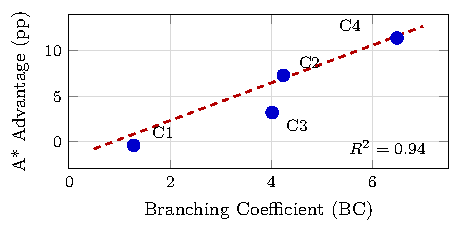
\includegraphics[width=0.85\columnwidth]{topology_scatter.pdf}
\caption{A* advantage (pp) vs.\ branching coefficient across topology clusters. Linear fit: $R^2=0.94$.}
\label{fig:topology_scatter}
\end{figure}

\paragraph{Prescriptive decision rule.}
The cluster analysis yields a practical decision rule: \emph{C1 (linear)}: use CoT; search overhead is unnecessary. \emph{C2 (mid-branch)}: route adaptively; this is where router quality matters most. \emph{C3 (complex, noisy)}: neither method is reliable; retrieval augmentation or stronger models may be needed. \emph{C4 (deep-branch)}: use A*; search has the clearest advantage.

\paragraph{Topic modelling validates topology.}
As independent validation, we apply Non-negative Matrix Factorisation (NMF, $k$=8) on TF-IDF representations of all 3,660 paired evaluation questions. A* dominates in 6 of 8 topic categories covering 66.2\% of the corpus---these share multi-hop entity chains (entertainment, historical events, geography, biography, politics). CoT-dominant topics (33.8\%) correspond to single-step commonsense categories (everyday reasoning, hypothetical scenarios). Full per-topic results with examples in Appendix~\ref{app:topics}.

%=============================================================================
\subsection{Topology-Aware Routing}
\label{sec:topology_routing}
%=============================================================================

Table~\ref{tab:topology_router} compares all routers and reports oracle gap recovery.



\begin{table}[t]
\centering
\small
\adjustbox{width=\textwidth}{
\begin{tabular}{llcccccccccc}
\toprule
\textbf{Router} & \textbf{Input}
& \textbf{Str.QA}
& \textbf{Log.QA}
& \textbf{Hot.QA}
& \textbf{GSM8K}
& \textbf{MATH}
& \textbf{HE}
& \textbf{MBPP}
& \textbf{CC}
& \textbf{Gap\%} \\
\midrule
A* only & traces
& 74.80 & 44.85 & 80.10 & 86.12 & 79.10 & 64.42 & 36.80 & 87.00 & $-$10.9 \\

CoT only & traces
& 64.52 & 45.78 & 76.80 & 85.04 & 78.00 & 67.48 & 39.80 & 77.40 & $-$24.6 \\
\midrule
Sem.\ Entropy & traces
& 74.37 & 47.47 & 81.30 & 86.67 & 78.24 & 65.64 & 37.00 & 88.20 & $-$3.9 \\

LLM-as-Critic & traces
& 74.19 & 47.16 & 80.21 & 87.28 & 79.13 & 71.17 & 40.20 & 97.80 & 9.6 \\

LLM-as-Judge & traces
& 73.28 & 47.21 & 80.87 & 85.65 & 78.23 & 71.78 & 40.40 & 97.80 & 6.6 \\

Random Forest & features
& 76.25 & 48.20 & 81.25 & 87.43 & 80.12 & 67.48 & 39.60 & 77.40 & $-$3.3 \\

\textbf{Topology Router} & \textbf{13 feat.}
& \textbf{77.35} & \textbf{49.01} & \textbf{82.41}
& \textbf{91.10} & \textbf{81.52} & \textbf{72.50} & \textbf{40.63} & \textbf{95.00} & \textbf{40.0} \\
\midrule
Oracle & --
& 84.59 & 59.29 & 94.20 & 96.14 & 84.17 & 74.85 & 44.00 & 96.20 & 100 \\
\bottomrule
\end{tabular}}
\caption{Router comparison on LLaMA-3.1-8B. HE = HumanEval, CC = CodeContests. Scores denote accuracy (\%). On CodeContests, the topology router achieves 95.0\% (vs.\ A*-only 87.0\%, oracle 96.2\%)---recovering 87\% of the oracle gap, the strongest single-dataset result. Gap\% to be recomputed with corrected CC data; SE/Critic/Judge on CC pending re-run. All QA router improvements over CoT: McNemar's $p<0.005$. LLM-as-Judge and LLM-as-Critic prompts in Appendix Figure~\ref{fig:judge_critic_prompts}.}
\label{tab:topology_router}
\end{table}



{
\begin{table}[ht]
\centering
\small
\adjustbox{width=\textwidth}{
\begin{tabular}{llccccccccc}
\toprule
\textbf{Router} & \textbf{Input}
& \textbf{Str.QA} & \textbf{Log.QA} & \textbf{Hot.QA}
& \textbf{GSM8K} & \textbf{MATH}
& \textbf{HE} & \textbf{MBPP} & \textbf{CC} & \textbf{Gap\%} \\
\midrule
\multicolumn{11}{c}{\textit{Qwen-2.5-14B}} \\
\midrule
A* only & traces & 74.72 & 57.45 & 82.50 & 80.59 & 47.20 & 76.07 & 45.00 & 94.40 & $-$7.5 \\
CoT only & traces & 75.98 & 57.30 & 56.20 & 61.56 & 43.80 & 77.91 & 46.60 & 99.60 & $-$78.0 \\
\midrule
Sem.\ Entropy & traces & 76.24 & 57.45 & 68.40 & 73.31 & 45.60 & 79.14 & 45.40 & 94.40 & $-$36.2 \\
LLM-as-Critic & traces & 75.98 & 57.45 & 82.50 & 70.13 & 44.20 & 75.46 & 48.80 & 95.20 & $-$21.9 \\
LLM-as-Judge & traces & 75.90 & 57.30 & 57.55 & 69.07 & 45.20 & 77.30 & 48.40 & 95.20 & $-$59.8 \\
Random Forest & features & 74.54 & 58.53 & 75.50 & 61.56 & 43.80 & 76.69 & 46.60 & 99.60 & $-$49.5 \\
\textbf{Topology Router} & \textbf{13 feat.} & \textbf{76.46} & \textbf{58.68} & \textbf{83.17} & \textbf{80.82} & \textbf{48.40} & \textbf{79.75} & 48.42 & -- & \textbf{11.9} \\
\midrule
Oracle & -- & 81.22 & 68.51 & 86.40 & 89.69 & 66.20 & 85.89 & 53.00 & 100.00 & 100 \\
\midrule
\multicolumn{11}{c}{\textit{Qwen-0.5B}} \\
\midrule
A* only & traces & 59.09 & 20.20 & 30.00 & 14.48 & 16.20 & 20.25 & 20.80 & 68.20 & $-$68.3 \\
CoT only & traces & 56.36 & 24.00 & 7.50 & 26.84 & 32.80 & 33.74 & 24.00 & 49.80 & $-$60.2 \\
\midrule
Sem.\ Entropy & traces & 56.36 & 24.00 & 12.50 & 26.84 & 20.20 & 21.47 & 22.40 & 65.20 & $-$68.6 \\
LLM-as-Critic & traces & 59.09 & 24.00 & 30.00 & 27.90 & 31.20 & 33.13 & 27.00 & 59.20 & $-$9.9 \\
LLM-as-Judge & traces & 58.18 & 32.40 & 32.50 & 27.37 & 32.20 & 34.97 & 27.20 & 55.60 & 2.4 \\
Random Forest & features & \textbf{61.82} & 21.20 & 25.00 & 26.84 & 32.60 & 33.74 & 24.00 & 64.40 & $-$12.5 \\
\textbf{Topology Router} & \textbf{13 feat.} & \textbf{64.74} & 24.98 & 30.00 & \textbf{26.84} & \textbf{33.21} & \textbf{34.97} & 25.99 & \textbf{75.20} & \textbf{25.6} \\
\midrule
Oracle & -- & 81.82 & 34.20 & 35.00 & 34.04 & 38.20 & 38.04 & 29.80 & 76.00 & 100 \\
\bottomrule
\end{tabular}}
\caption{Router comparison at 14B and 0.5B scales. HE = HumanEval, CC = CodeContests. The topology router is highest on most datasets at both scales; at 0.5B it recovers 89.7\% of the CodeContests oracle gap using only problem text. -- indicates data not yet available.}
\label{tab:router_14b_05b}
\end{table}


\textbf{Why pre-generation routing outperforms post-hoc routing.}
The topology router observes no generated traces, yet outperforms routers that inspect both full reasoning traces. This reverses the intuitive expectation that seeing full traces should be more informative. The bottleneck is often not judging which completed trace looks better, but recognizing before generation which computation the problem requires. The same holds for code: on HumanEval (8B), the topology router reaches 72.5\% vs.\ 71.8\% for LLM-as-Judge, and on CodeContests (0.5B) it recovers 89.7\% of the oracle gap---both without seeing any generated code (Table~\ref{tab:router_14b_05b}, Appendix~\ref{app:code_generation}).

\textbf{Fluency-Correctness Asymmetry.}
We identify a fundamental limitation of output-based routing: in 38\% of disagreement cases, CoT produces the \emph{more fluent} trace but the \emph{wrong} answer (Table~\ref{tab:fluency_asymmetry}). A critic that rewards coherence can therefore prefer the wrong computation. This asymmetry explains why the topology router (which sidesteps trace evaluation entirely) outperforms the LLM-as-critic.

\textbf{Feature ablation: reasoning structure vs.\ surface statistics.}
To verify that the topology router captures genuine reasoning structure rather than surface artifacts, we evaluate feature subsets (Table~\ref{tab:feature_ablation}). Strikingly, using only the 9 reasoning-structure features (connectives, negation, hops, comparisons, linearity, depth, branching complexity, BC)---\emph{excluding} all length and format features---\textbf{improves} router performance from 71.8\% to 75.0\% CV accuracy (Gap: 41.9\% $\to$ 48.5\%). This demonstrates that the topology router's predictive power comes from reasoning-structural properties, not from length or format statistics that might encode dataset identity.

\begin{table}[ht]
\centering
\small
\begin{tabular}{lcc}
\toprule
\textbf{Feature Set} & \textbf{CV Accuracy} & \textbf{Gap\%} \\
\midrule
All 14 features & 0.718 & 41.9 \\
\textbf{Reasoning only (9 features)} & \textbf{0.750} & \textbf{48.5} \\
Format only (5 features) & 0.713 & 40.8 \\
No length features (12) & 0.717 & 41.6 \\
BC only (1 feature) & 0.709 & 40.0 \\
Top-5 reasoning features & 0.745 & 47.4 \\
\bottomrule
\end{tabular}
\caption{Feature ablation on pooled 8B data (6 benchmarks, 2660 instances). Reasoning-only features (connectives, negation, hops, comparisons, depth, BC) outperform the full set, confirming that the router learns reasoning structure, not surface statistics.}
\label{tab:feature_ablation}
\end{table}

\begin{table}[t]
\centering
\small
\begin{tabular}{lcc}
\toprule
\textbf{Metric} & \textbf{A*} & \textbf{CoT} \\
\midrule
Average fluency score & 0.725 & 0.673 \\
Cases where more fluent & 62.0\% & 38.0\% \\
More-fluent but wrong & \multicolumn{2}{c}{38.0\% of disagreements} \\
\bottomrule
\end{tabular}
\caption{Fluency-Correctness Asymmetry on disagreement cases. Trace fluency does not predict correctness.}
\label{tab:fluency_asymmetry}
\end{table}

%=============================================================================
\subsection{Sensitivity, Compute, and Failure Analysis}
\label{sec:sensitivity}
%=============================================================================

\textbf{Sensitivity analysis.}
On a stratified 300-question HotpotQA sample (seed=42), we sweep the node budget $B \in \{5,10,15,20,30\}$ and branching factor $K \in \{1,2,3,4\}$ (full tables in Appendix~\ref{app:sensitivity}). Accuracy improves from $B$=5 (73.0\%) to $B$=20 (78.7\%), then drops at $B$=30 (76.0\%), indicating diminishing returns. The default $B$=15 (78.0\%) lies within 0.7\,pp of the peak. Even $K$=1 (no real branching) achieves 77.7\%, confirming graceful degradation and exceeding self-consistency.

\textbf{Compute--accuracy tradeoff.}
A* at the default ($K$=3, $B$=15) uses $\sim$12,452 measured tokens/question ($\sim$24$\times$ CoT's $\sim$512). A budget-reduced variant ($K$=1) achieves competitive accuracy at 3,372 tokens/question ($\sim$7$\times$ CoT). A* is substantially more expensive; its use is justified only when topology predicts branching is useful, motivating pre-routing as a compute-saving mechanism (full table in Appendix~\ref{app:compute}).

\textbf{Failure analysis.}
Among A* failures on instances CoT solves correctly, 91.1\% are \emph{overthinking} (search continues past correct evidence, accumulating distractors) and 8.9\% are \emph{premature commitment} (search locks onto an early branch). CoT fails by committing too early; A* fails by continuing too long. The same branching mechanism that helps on multi-hop problems hurts on linear ones (examples in Appendix~\ref{app:astar_failures}).

\textbf{Human evaluation.} We conduct a human evaluation of reasoning-trace quality using the criteria in \S\ref{annot-crit}. Two post-graduate annotators with experience in LLM reasoning research each labeled 100 instances from StrategyQA and LogicQA. Across datasets and metrics, Cohen's \(\kappa\) ranges from 0.59 to 0.68, indicating fair agreement. Two annotators labeled 100 disagreement instances per dataset on \emph{coverage} (1--3) and \emph{relevance} (1--3), with Cohen's $\kappa$: 0.59--0.68. The correct method consistently achieves higher coverage (e.g., StrategyQA: CoT-correct 3.00 vs.\ A* 1.20; A*-correct 2.71 vs.\ CoT 1.63), confirming that disagreements are driven by coverage of the required reasoning path rather than surface quality (full results in Appendix~\ref{app:human_eval}).









% \subsection{Human evaluation}
% We perform a human evaluation to assess the quality and richness of the reasoning trace (desribed below \S \ref{annot-crit}). Two post-graduate students with adequate experience in LLM reasoning research were employed to annotate 100 instances from LogicQA and StrategyQA each. Across datasets and metrics, inter-annotator agreement score as measured by Cohen's kappa ranges from 0.59 to 0.68, which denotes a fair agreement.



% \noindent\textbf{Interpretation.}
% Across both StrategyQA and LogicQA, the method that is correct on a disagreement case almost always receives a substantially higher \emph{coverage} score than the method that is wrong. On StrategyQA, when CoT is correct and A* is wrong, CoT attains perfect average coverage (3.00) while A* drops to 1.20; when A* is correct and CoT is wrong, A* rises to 2.71 while CoT remains at 1.63. The same pattern holds on LogicQA (3.00 vs.\ 1.86 for CoT-right cases, and 2.77 vs.\ 1.88 for A*-right cases). This suggests that disagreement cases are primarily explained by \emph{coverage of the required reasoning path}, rather than by superficial stylistic differences.


% \noindent\textbf{Annotation criteria.}\label{annot-crit}
% \textit{Coverage} measures whether a reasoning trace meaningfully reaches the required inferential path and supports the final conclusion. We score coverage on a 3-point scale: 1 if the reasoning is mostly incorrect and does not reach the conclusion, 2 if it is mostly correct but still fails to reach the final conclusion, and 3 if the reasoning is correct and the final conclusion is also correct.

% \noindent\textit{Relevance} measures how focused the reasoning steps are on concepts that are actually needed for answering the question. We operationalize it as a coarse 3-point judgment based on the proportion of relevant steps among all steps, where relevant steps are those that stay on-topic and do not introduce unnecessary concepts not motivated by the question.

% \noindent Relevance shows a weaker and less consistent pattern. In StrategyQA, CoT tends to remain more relevant than A* when both are wrong (2.82 vs.\ 1.55), whereas in LogicQA both methods maintain moderately high relevance even when incorrect (2.76 for CoT and 2.53 for A*). Thus, being on-topic is not sufficient for correctness: a trace can stay locally relevant yet still fail to cover the crucial inferential steps needed for the final answer. Overall, the annotations indicate that the main difference between CoT and A* on disagreement cases lies in \emph{which method better covers the decisive reasoning steps}, while relevance is more weakly associated with answer correctness.
%=============================================================================







\section{Related Work}
\label{sec:related}
%=============================================================================

\paragraph{CoT and structured reasoning.}
Chain-of-thought prompting~\cite{wei2022chain} reasons through a single linear trace, while self-consistency~\cite{wang2022self}, Tree-of-Thoughts~\cite{yao2024tree}, and Graph-of-Thoughts~\cite{besta2024graph} add sampling, tree search, or graph-structured deliberation. Prior work mostly asks whether richer reasoning structures improve aggregate accuracy, and recent work shows that CoT itself is not uniformly beneficial~\cite{meincke2025cot}. We ask the complementary question: when does moving from linear reasoning to search help, and when does it hurt?

\paragraph{Search-augmented reasoning and inference-time compute.}
MCTS-style reasoning~\cite{hao2023reasoning}, beam search~\cite{xie2024self}, LATS~\cite{zhou2024lats}, MCTSr~\cite{zhang2024mctsrmath}, and rStar-Math~\cite{guan2025rstar} demonstrate the value of explicit exploration. \cite{snell2024scaling} show that scaling test-time compute can be more effective than scaling parameters, but leave open the question of \emph{which} problems benefit from additional compute. Self-Refine~\cite{madaan2023selfrefine} and reasoning-focused models like DeepSeek-R1~\cite{deepseekr1} allocate variable compute adaptively, but do not provide pre-generation prediction of when this helps. We use A* as a controlled diagnostic and show that search gains are topology-dependent: branching, multi-hop, and hypothesis-elimination problems benefit most, while simpler linear cases can degrade.

\paragraph{Over-exploration and search failures.}
Work on overthinking and excessive reasoning often treats over-exploration as an efficiency issue~\cite{sui2025overthinking,wang2025fetch,ma2025cotvalve}, and \cite{wang-etal-2025-dont} identify over- and under-exploration as dual pitfalls of tree search. We show the problem is also one of correctness: 91.1\% of A* failures on CoT-correct instances arise from overthinking, where search continues beyond sufficient evidence, accumulates distractors, or revisits near-duplicate states.

\paragraph{Routing and critic limitations.}
Semantic entropy~\cite{kossen2024semanticentropyprobesrobust}, LLM-as-judge methods~\cite{zheng2023judging}, and process supervision~\cite{lightman2023let} rely on generated traces to assess reasoning quality, while mixture-of-experts models~\cite{shazeer2017outrageouslylargeneuralnetworks} route between neural modules. We instead route between \emph{reasoning algorithms} before generation, using input topology (Table~\ref{tab:method_comparison}). This is crucial because our Fluency--Correctness Asymmetry shows that fluent traces can be wrong: in 38\% of disagreement cases, the more fluent trace gives the incorrect answer. Our contribution is a diagnostic framework for deciding \emph{when} search should be used.


\begin{table}[t]
\centering
\scriptsize
\setlength{\tabcolsep}{2.5pt}
\begin{tabular}{lccccp{1.8cm}}
\toprule
\textbf{Method} & \textbf{Structure} & \textbf{Front.} & \textbf{Heur.} & \textbf{Pre-rte} & \textbf{Limitation} \\
\midrule
CoT & linear & \ding{55} & \ding{55} & \ding{55} & premature commit \\
SC & multi-linear & \ding{55} & \ding{55} & \ding{55} & unguided sampling \\
ToT & tree/BFS & \ding{51} & eval. & \ding{55} & evaluator entangled \\
MCTS & tree+rollout & \ding{51} & value & \ding{55} & many design choices \\
A* (ours) & priority & \ding{51} & \ding{51} & \ding{51} & higher compute \\
\bottomrule
\end{tabular}
\caption{Methodological comparison of reasoning strategies. Front.\ = explicit frontier; Heur.\ = heuristic guidance; Pre-rte = pre-generation routing studied. A* isolates the role of heuristic-guided search without entangling evaluator design or rollout policy.}
\label{tab:method_comparison}
\end{table}

\section{Conclusion}
Across eight benchmarks---spanning QA, math, and code generation---and three model scales, we find that CoT and A* are complementary rather than hierarchical: the gap between the oracle and the best single method is consistently large. The key explanatory variable is branching coefficient, not dataset identity---a structural finding that holds across all three domains. Perhaps most surprisingly, a router that sees only the raw input (no traces) outperforms critics that inspect both full reasoning chains, because trace fluency misleads post-hoc judges in a systematic way. Code generation exhibits the same pattern: on CodeContests at 8B, the topology router reaches 95.0\% accuracy (vs.\ A*-only 87.0\%), recovering 87\% of the oracle gap---the strongest single-dataset result. At 0.5B, A* gives +18.4\,pp on CodeContests, and the overall 8B gap recovery across all eight benchmarks reaches 40.0\%. These results suggest that the next step for adaptive inference is not better trace evaluation but better problem-structure recognition. Concrete next steps include learned topology embeddings and code-specific structural features (e.g., AST complexity, specification ambiguity).

\section*{Limitations}
\label{sec:limitations}
Our findings are conditioned on a single budgeted A* implementation; a different search policy (MCTS, beam search) could shift where the complementarity boundary lies. The 13 topology features are hand-designed proxies---interpretable but unlikely to capture the full latent structure of reasoning difficulty. They also rely on English-language parsing tools, limiting direct transfer to other languages or code. The critic-based heuristic depends on DeepSeek-R1-Distill-Qwen-14B; although the topology router reduces this dependence, it does not eliminate it entirely. On the cost side, A* at default settings uses $\sim$24$\times$ the tokens of CoT, and our token accounting covers only a 300-question ablation sample. Domain coverage spans QA, math, and code generation; long-form generation remains untested. On code tasks, the NL-oriented topology features work well on HumanEval (rich specifications) but degenerate on MBPP (ultra-short prompts); code-specific topology features (e.g., AST complexity, edge-case count) remain future work. Finally, the topology router is an XGBoost classifier on fixed features; a learned router that jointly optimizes routing and search would be a natural next step.

\bibliographystyle{acl_natbib}
\bibliography{custom}













% \end{thebibliography}

%-----------------------------------------------------------------------------
\appendix
%-----------------------------------------------------------------------------

% \section{Auxiliary Conservative Heuristic Construction}
% \label{app:auxiliary_heuristic}

% This appendix presents a formal admissibility proof for an auxiliary depth-plus-coverage heuristic. This construction applies to a simplified setting and is \emph{not} used as the main experimental heuristic (which is the critic-based heuristic described in Section~\ref{sec:heuristic}). We include it for theoretical completeness.


































\section{More on admissibility and generalizability of the heuristics}\label{more-on}

\paragraph{Admissibility and consistency.}
Under the minimum-hop and non-goal-continuation assumptions, this
heuristic is admissible when its weights are bounded by the minimum
transition cost. In our implementation, \(H_{\min}=2\),
\(\omega_d=\omega_c=0.3\), and \(c_{\max}=0.99\), so the minimum
transition cost is
\[
c_{\min}=1+(1-c_{\max})=1.01.
\]
The largest possible heuristic value at the root is
\[
2\omega_d+\omega_c=0.9,
\]
which is below the minimum two-step path cost \(2c_{\min}=2.02\). After
one step, the heuristic is at most \(\omega_d+\omega_c=0.6<c_{\min}\),
and after the minimum-hop threshold the coverage term is at most
\(\omega_c=0.3<c_{\min}\). Hence the heuristic lower-bounds the remaining
path cost under the stated assumptions and is admissible. It is also
consistent, since a single transition can reduce the heuristic by at most
\(\omega_d+\omega_c=0.6\), which is smaller than the minimum transition
cost \(c_{\min}=1.01\).

\begin{algorithm}[t]
\caption{Dataset-Agnostic Symbolic Progress Heuristic}
\label{alg:symbolic-progress-heuristic}
\KwIn{
Question \(q\); partial reasoning state \(n=(\tau_n,d_n)\);
minimum-hop lower bound \(H_{\min}\); weights \(\omega_d,\omega_c\)
}
\KwOut{Heuristic value \(h(n)\)}

\BlankLine
\textbf{Step 1: Extract question content units.}\;
Initialize \(\mathcal{E}_q \leftarrow \emptyset\).\;
Add all quoted strings in \(q\) to \(\mathcal{E}_q\).\;
Add all proper-name phrases in \(q\) to \(\mathcal{E}_q\).\;
Add all numbers and years in \(q\) to \(\mathcal{E}_q\).\;
Add all non-stopword content terms of length greater than three to \(\mathcal{E}_q\).\;

\BlankLine
\textbf{Step 2: Compute entity/content coverage.}\;
\If{\(\mathcal{E}_q=\emptyset\)}{
    \(E(n) \leftarrow 1\)\;
}
\Else{
    \(C(n) \leftarrow \{e\in\mathcal{E}_q : e \text{ appears in } \tau_n\}\)\;
    \(E(n) \leftarrow \frac{|C(n)|}{|\mathcal{E}_q|}\)\;
}

\BlankLine
\textbf{Step 3: Compute remaining structural progress.}\;
\(r_{\mathrm{depth}}(n) \leftarrow \max(0,H_{\min}-d_n)\)\;
\(h_{\mathrm{depth}}(n) \leftarrow \omega_d r_{\mathrm{depth}}(n)\)\;

\BlankLine
\textbf{Step 4: Compute remaining content progress.}\;
\(h_{\mathrm{coverage}}(n) \leftarrow \omega_c(1-E(n))\)\;

\BlankLine
\textbf{Step 5: Return total heuristic.}\;
\(h(n) \leftarrow h_{\mathrm{depth}}(n)+h_{\mathrm{coverage}}(n)\)\;
\Return \(h(n)\)\;
\end{algorithm}

\paragraph{Human validation of heuristic progress.}
We additionally validate whether the symbolic progress heuristic behaves
conservatively on intermediate reasoning states. We sample 500 partial
states produced during A* search and ask human annotators to assign a
normalized progress score indicating how close the partial trace is to a
valid answer. The model used is LLaMA-3.1-8B and the datasets are 100 StrategyQA, 100 HotpotQA, and 300 LogicQA. We then compare this human-assessed progress with the
heuristic's implied progress score. The heuristic underestimates progress
on average (0.43 vs. 0.58, paired \(t\)-test \(p<0.001\)), with an
overestimation rate of 12.3\% and maximum observed overestimation
\(\epsilon_{\max}=0.14\). Thus, the heuristic is conservative in
expectation: it tends not to overstate the completeness of a partial
trace. This supports its use as a safe search-control signal rather than
as an unconstrained learned verifier.


















\section{Qualitative Examples}
\label{app:qualitative_examples}

This appendix provides the detailed examples corresponding to the qualitative conclusions summarized in Section~\ref{sec:qualitative_conclusions}.

\subsection{Patterns of A* Success and CoT Failure}
\label{app:astar_success}

We identify three recurring settings where A* succeeds while CoT fails.

\paragraph{Group 1: Non-linear evidence aggregation.}
These are questions where the answer requires combining several facts that do not naturally form a single left-to-right narrative.

\begin{examplebox}[title=StrategyQA --- Non-linear Evidence Aggregation]
\textbf{Q:} \emph{Is shrimp scampi definitely free of plastic?} \quad (Gold: \textsc{No})
\tcblower
\textbf{CoT} ($\times$ predicts \textsc{Yes}): Proceeds through five sequential steps analyzing harvesting, processing, cooking, ingredients, and regulations. Each step independently concludes no significant plastic risk. The linear structure prevents cross-referencing marine biology evidence with the food preparation chain.\\[4pt]
\textbf{A*} ($\checkmark$ predicts \textsc{No}): Step 1 directly identifies microplastic bioaccumulation in shrimp tissue. Step 2 notes that cooking does not remove microplastics. The heuristic guides the search toward the most relevant evidence node, avoiding the exhaustive but misleading step-by-step analysis.
\end{examplebox}

\begin{examplebox}[title=LogicQA --- Non-linear Evidence Aggregation]
\textbf{Q:} \emph{Based on the above statement [spatial arrangement of communities around Civic Park], which of the following can be derived?} \quad (Gold: A)
\tcblower
\textbf{CoT} ($\times$ predicts D): Analyzes spatial relationships sequentially, accumulating errors in relative positioning. By the fourth step, the accumulated imprecision leads to selecting an incorrect spatial relationship.\\[4pt]
\textbf{A*} ($\checkmark$ predicts A): Explores multiple spatial constraint combinations in parallel. The search finds a consistent assignment by simultaneously satisfying the ``southwest of'' and ``southeast of'' constraints, correctly deriving that Civic Park is north of the administrative service area.
\end{examplebox}

\paragraph{Group 2: Hypothesis elimination.}
A* is also effective when the problem naturally decomposes into evaluating or eliminating alternatives.

\begin{examplebox}[title=LogicQA --- Hypothesis Elimination]
\textbf{Q:} \emph{Which of the following is most similar to the argument: ``All landscape rooms can see the landscape, but Li Wenbing's family can't see the landscape. Therefore, Li Wenbing's family is not a landscape room.''} \quad (Gold: D)
\tcblower
\textbf{CoT} ($\times$ predicts C): Identifies the logical structure (modus tollens) but then incorrectly maps it to option C (a modus ponens structure) due to surface similarity.\\[4pt]
\textbf{A*} ($\checkmark$ predicts D): Separately evaluates options through different branches. One branch identifies the negative inference pattern in the premise and correctly maps it to option D (``Anyone who meets conditions can apply; Sun Wen did not apply; therefore Sun Wen did not meet conditions''), which preserves the modus tollens structure.
\end{examplebox}

\paragraph{Group 3: Multi-hop question answering.}
HotpotQA highlights the value of search when the answer depends on chaining facts across sources.

\begin{examplebox}[title=HotpotQA --- Multi-hop Chaining]
\textbf{Q:} \emph{What government position was held by the woman who portrayed Corliss Archer in the film \textit{Kiss and Tell}?} \quad (Gold: Chief of Protocol)
\tcblower
\textbf{CoT} ($\times$ predicts ``Ambassador''): Correctly identifies Shirley Temple as the actress but then retrieves an incorrect government position from parametric memory, confusing ambassadorial roles with her protocol role.\\[4pt]
\textbf{A*}: Explores multiple evidence paths for Shirley Temple's government career. While the trace is imperfect, the tree search structure allows it to consider multiple candidate positions before committing.
\end{examplebox}

\subsection{Patterns of CoT Success and A* Failure}
\label{app:cot_success}

We identify two common settings where CoT remains better than search.

\paragraph{Group 1: Direct factual reasoning.}
When the answer follows directly from familiar facts, search can introduce unnecessary branching and semantic drift.

\begin{examplebox}[title=StrategyQA --- Direct Factual Reasoning]
\textbf{Q:} \emph{Is a Boeing 737 cost covered by \textit{Wonder Woman} (2017 film) box office receipts?} \quad (Gold: \textsc{Yes})
\tcblower
\textbf{CoT} ($\checkmark$ predicts \textsc{Yes}): Directly retrieves the production budget ($\sim$\$150M), box office ($\sim$\$822M), and Boeing 737 cost ($\sim$\$100M), concluding that the receipts exceed the aircraft cost.\\[4pt]
\textbf{A*} ($\times$ predicts \textsc{No}): The first search step focuses on whether box office receipts are ``associated with'' aircraft purchases, misreading the question as one about financial transactions rather than magnitude comparison.
\end{examplebox}

\begin{examplebox}[title=StrategyQA --- Direct Factual Reasoning]
\textbf{Q:} \emph{Is average number of peas in a pod enough commas for a billion?} \quad (Gold: \textsc{Yes})
\tcblower
\textbf{CoT} ($\checkmark$ predicts \textsc{Yes}): Correctly identifies that a billion (1,000,000,000) requires three commas and that a pea pod usually contains 7--9 peas, so the answer is yes.\\[4pt]
\textbf{A*} ($\times$ predicts \textsc{No}): Incorrectly states that a billion has 12 zeros and becomes confused by the scale comparison.
\end{examplebox}

\paragraph{Group 2: Fluent world knowledge and argumentation.}
When the problem is best solved by a smooth, coherent narrative, CoT often remains more reliable than fragmented search steps.

\begin{examplebox}[title=LogicQA --- Fluent Argumentation]
\textbf{Q:} \emph{Which of the following is the best argument against the claim that rich Chinese are transferring property abroad?} \quad (Gold: B)
\tcblower
\textbf{CoT} ($\checkmark$ predicts B): Systematically compares the answer options and identifies the strongest counterargument.\\[4pt]
\textbf{A*} ($\times$ predicts A): The first search step identifies option A as relevant, and the heuristic keeps the search near that branch without sufficiently comparing the full option set.
\end{examplebox}

\subsection{A* Failure Modes on Simple Cases}
\label{app:astar_failures}

We observe three recurrent failure modes for A* on examples that CoT solves easily.

\paragraph{Failure mode 1: Overthinking simple questions.}

\begin{examplebox}[title=StrategyQA --- Overthinking]
\textbf{Q:} \emph{Does Disney have an ice princess?} \quad (Gold: \textsc{Yes})
\tcblower
\textbf{A*} ($\times$ predicts \textsc{No}): Step 1 correctly identifies Elsa from \emph{Frozen} as having ice powers. Step 2 notes that she is called ``The Ice Queen'' in promotional material. The search then turns the easy recall problem into an unnecessary semantic distinction between ``queen'' and ``princess,'' yielding the wrong answer.
\end{examplebox}

\paragraph{Failure mode 2: Spurious correlations in search.}

\begin{examplebox}[title=StrategyQA --- Spurious Correlation]
\textbf{Q:} \emph{Is Menthol associated with Thanksgiving?} \quad (Gold: \textsc{No})
\tcblower
\textbf{A*} ($\times$ predicts \textsc{Yes}): Step 1 associates menthol with cough drops used in cold weather. Step 2 associates Thanksgiving with cold weather in North America. Step 3 turns these weak associations into a spurious chain, effectively reasoning menthol $\rightarrow$ cold weather $\rightarrow$ Thanksgiving.
\end{examplebox}

\paragraph{Failure mode 3: Step repetition.}

\begin{examplebox}[title=StrategyQA --- Step Repetition]
\textbf{Q:} \emph{Will the Albany in Georgia reach a hundred thousand occupants before the one in New York?} \quad (Gold: \textsc{No})
\tcblower
\textbf{A*} ($\times$ predicts \textsc{Yes}): Step 2 states the population of Albany, New York ($\sim$98{,}000). Step 3 largely repeats the same fact. The repetition wastes node budget that should have been used to compare growth trajectories.
\end{examplebox}


\begin{algorithm}[t]
\caption{Budgeted A* Search over Reasoning Traces}
\label{alg:astar}
\begin{algorithmic}[1]
\REQUIRE Problem $\mathcal{Q}=(q,C,\mathcal{O})$, model $\mathcal{M}_\theta$, depth limit $D_{\max}$, node budget $B$, candidates $N_c$
\STATE Initialize root $n_0 \gets (\emptyset,0)$, $g(n_0) \gets 0$, $h(n_0) \gets h(n_0)$ from the heuristic (Section~\ref{sec:heuristic_design})
\STATE $\textsc{Open} \gets \{n_0\}$ (priority queue on $f(n)=g(n)+h(n)$)
\STATE $\textsc{Visited} \gets \emptyset$, $\textsc{Goals} \gets \emptyset$, explored $\gets 0$
\WHILE{$\textsc{Open} \neq \emptyset$ and explored $< B$}
    \STATE $n \gets \textsc{Open}.\text{pop\_min}()$
    \IF{$\text{sig}(n) \in \textsc{Visited}$}
        \STATE continue
    \ENDIF
    \STATE $\textsc{Visited} \gets \textsc{Visited} \cup \{\text{sig}(n)\}$
    \STATE explored $\gets$ explored $+ 1$
    \IF{$\textsc{IsGoal}(n)$}
        \STATE $\textsc{Goals} \gets \textsc{Goals} \cup \{n\}$
        \STATE continue
    \ENDIF
    \IF{$d_n \geq D_{\max}$}
        \STATE continue
    \ENDIF
    \STATE $\{(s^{(j)}, c^{(j)})\}_{j=1}^{N_c} \gets \textsc{GenerateSteps}(\mathcal{M}_\theta, q, C, \mathcal{O}, \tau_n, N_c)$
    \FOR{each $(s^{(j)}, c^{(j)})$}
        \STATE $n' \gets (\tau_n \oplus s^{(j)}, d_n+1)$
        \STATE $g(n') \gets g(n) + 1 + (1-c^{(j)})$
        \STATE $\textsc{Open}.\text{push}(n', g(n') + h(n'))$
    \ENDFOR
\ENDWHILE
\STATE \textbf{return} weighted vote over $\textsc{Goals}$
\end{algorithmic}
\end{algorithm}




\begin{figure}[t]
\centering
\small

% ---------- STYLE ----------
\tcbset{
  promptcard/.style={
    enhanced,
    colback=white,
    colframe=black!75,
    colbacktitle=black!6,
    coltitle=black,
    boxrule=0.7pt,
    arc=2mm,
    left=6pt,right=6pt,top=5pt,bottom=5pt,
    fonttitle=\bfseries\small,
    titlerule=0pt
  }
}

\begin{minipage}[t]{0.485\textwidth}
\begin{tcolorbox}[promptcard,title=LLM-as-Judge]
\textbf{Purpose.} Compare two candidate reasoning trajectories and decide which one solves the query more \emph{faithfully} and \emph{correctly}. 

\vspace{2pt}
\textbf{Inputs.}
\begin{itemize}
    \setlength{\itemsep}{1pt}
    \item Context
    \item Query
    \item Path A reasoning trace
    \item Path B reasoning trace
\end{itemize}

\vspace{-2pt}
\textbf{Evaluation criteria.}
\begin{itemize}
    \setlength{\itemsep}{1pt}
    \item \textbf{Faithfulness:} uses only the provided context and avoids invented constraints
    \item \textbf{Logical validity:} each step follows causally and coherently from prior steps
    \item \textbf{Grounded conclusion:} the final answer directly resolves the query from the established reasoning
\end{itemize}

\vspace{-2pt}
\textbf{Required output.}
The model first reasons internally about both traces, then returns only the winning path in constrained XML:
\begin{center}
\ttfamily
<winner>A</winner> \quad or \quad <winner>B</winner>
\end{center}
\end{tcolorbox}
\end{minipage}
\hfill
\begin{minipage}[t]{0.485\textwidth}
\begin{tcolorbox}[promptcard,title=LLM-as-Critic]
\textbf{Purpose.} Diagnose the weaknesses of two reasoning traces and determine which trace is better overall.

\vspace{2pt}
\textbf{Inputs.}
\begin{itemize}
    \setlength{\itemsep}{1pt}
    \item Question
    \item Answer options
    \item Trace A with predicted answer
    \item Trace B with predicted answer
\end{itemize}

\vspace{-2pt}
\textbf{Evaluation criteria.}
\begin{itemize}
    \setlength{\itemsep}{1pt}
    \item whether the reasoning actually entails the predicted answer
    \item whether there are logical fallacies or unsupported jumps
    \item whether any claims are hallucinated or ungrounded
\end{itemize}

\vspace{-2pt}
\textbf{Required output.}
The model returns a structured JSON critique with flaws for both traces and the preferred trace:
\begin{center}
\ttfamily
\{"trace\_A\_flaws": "...",\\
"trace\_B\_flaws": "...",\\
"better\_trace": "A/B"\}
\end{center}
\end{tcolorbox}
\end{minipage}

\vspace{2pt}
\caption{LLM-based routing prompts. The \emph{judge} prompt is verdict-oriented: it compares two reasoning paths under faithfulness and logical soundness criteria and outputs only the winner. The \emph{critic} prompt is diagnosis-oriented: it identifies flaws in each trace before selecting the better one in structured JSON form.}
\label{fig:judge_critic_prompts}
\end{figure}




\subsection{Human evaluation}\label{app:human_eval}
We conduct a human evaluation of reasoning-trace quality using the criteria in \S\ref{annot-crit}. Two post-graduate annotators with experience in LLM reasoning research each labeled 100 instances from StrategyQA and LogicQA (Table~\ref{tab:disagreement-pool}). Across datasets and metrics, Cohen's \(\kappa\) ranges from 0.59 to 0.68, indicating fair agreement.


\noindent\textbf{Annotation criteria.}\label{annot-crit}
\textit{Coverage} measures whether a trace reaches the required inferential path and supports the final conclusion. We use a 3-point scale: 1 if the reasoning is mostly incorrect and does not reach the conclusion, 2 if it is mostly correct but still fails to reach the conclusion, and 3 if both the reasoning and conclusion are correct.

\noindent\textit{Relevance} measures how focused the trace is on concepts actually needed to answer the question. We score it coarsely on a 3-point scale based on the proportion of relevant steps, where relevant steps remain on-topic and avoid introducing unnecessary concepts.

\noindent Relevance is less diagnostic. In StrategyQA, CoT remains more relevant than A* when both are wrong (2.82 vs.\ 1.55), while in LogicQA both methods stay moderately relevant even when incorrect (2.76 for CoT, 2.53 for A*). Thus, staying on-topic is not enough: a trace may remain relevant yet still miss the decisive inferential steps. Overall, the annotations indicate that the main difference between CoT and A* on disagreement cases lies in \emph{which method better covers the decisive reasoning steps}, while relevance is only weakly associated with correctness.


\noindent\textbf{Interpretation.}
Refer to Table \ref{tab:disagreement-human-eval}. Across both datasets, the method that is correct on a disagreement case consistently receives a much higher \emph{coverage} score than the method that is wrong. On StrategyQA, when CoT is correct and A* is wrong, CoT achieves average coverage 3.00 versus 1.20 for A*; when A* is correct and CoT is wrong, A* scores 2.71 versus 1.63 for CoT. The same pattern holds on LogicQA (3.00 vs.\ 1.86 for CoT-correct cases, and 2.77 vs.\ 1.88 for A*-correct cases). This suggests that disagreement cases are driven mainly by \emph{coverage of the required reasoning path}, not by superficial stylistic differences.

\begin{table}[t]
\centering
\small
\begin{tabular}{lrr}
\toprule
Dataset & \# disagreement cases & Annotation sample \\
\midrule
StrategyQA & 587 & 100 \\
LogicQA     & 332 & 100 \\
\bottomrule
\end{tabular}
\caption{Size of the disagreement pool used for human-style analysis. We consider only instances where CoT and A* produce different final predictions. In single-label QA, the \textit{both-right} bucket is therefore expected to be empty, which is confirmed in both datasets.}
\label{tab:disagreement-pool}
\end{table}

\begin{table}[t]
\centering
\small
\begin{tabular}{llrrrrr}
\toprule
Dataset & Correctness group & $n$ & CoT Cov. & CoT Rel. & A* Cov. & A* Rel. \\
\midrule
\multirow{3}{*}{StrategyQA}
& both wrong            & 11 & 1.00 & 2.82 & 1.09 & 1.55 \\
& CoT right, A* wrong   & 51 & 3.00 & 2.57 & 1.20 & 2.16 \\
& CoT wrong, A* right   & 38 & 1.63 & 2.47 & 2.71 & 2.00 \\
\midrule
\multirow{3}{*}{LogicQA}
& both wrong            & 38 & 1.79 & 2.76 & 1.89 & 2.53 \\
& CoT right, A* wrong   & 36 & 3.00 & 2.81 & 1.86 & 2.47 \\
& CoT wrong, A* right   & 26 & 1.88 & 2.81 & 2.77 & 2.42 \\
\bottomrule
\end{tabular}
\caption{Human-style annotation on 100 sampled disagreement cases per dataset. “Cov.” denotes reasoning coverage (1--3), and “Rel.” denotes relevance (1--3). Coverage measures whether the reasoning substantially reaches a correct conclusion; relevance measures the proportion of steps that stay on-topic and avoid unnecessary concepts.}
\label{tab:disagreement-human-eval}
\end{table}




% \section{Human Evaluation Details}
% \label{app:human_eval}

% Two annotators labeled 100 disagreement instances per dataset on \emph{coverage} (1--3: does the trace reach the required inferential path?) and \emph{relevance} (1--3: stays on-topic?). Cohen's $\kappa$: 0.59--0.68.


% The correct method consistently receives higher coverage. Relevance is weakly diagnostic: a trace can stay on-topic yet miss decisive steps.

\section{FAQs}
\label{app:faqs}

\paragraph{Q1. Why are gains on HotpotQA larger than StrategyQA?}
HotpotQA explicitly rewards multi-hop evidence aggregation; StrategyQA is often solvable linearly.

\paragraph{Q2. Why include LogicQA where A* underperforms?}
LogicQA stresses formal sequential reasoning where branching can interfere, giving a more honest picture.

\paragraph{Q3. How reliable are self-reported confidence scores?}
They are pragmatic ranking signals (not calibrated probabilities) biasing search toward shorter, more confident traces.

\paragraph{Q4. How should readers interpret the admissibility result?}
The formal proof (Appendix~\ref{full-proof}) applies only to the auxiliary depth-coverage heuristic under explicit assumptions. The main experimental heuristic is empirically validated (Appendix Section~\ref{more-on}) and also formally admissible.

\paragraph{Q5. Would ensemble voting capture the same complementarity?}
Only partially. Self-consistency recovers diversity but does not guide exploration toward promising reasoning states.

\paragraph{Q6. Is goal detection based on answer patterns brittle?}
Somewhat. Pattern matching is fast and reproducible but can miss valid conclusions phrased differently.

\section{Sensitivity Analysis}
\label{app:sensitivity}

All experiments are performed on a fixed stratified 300-question HotpotQA sample (seed=42). The results for budget sweep and branching factor sweep are depicted in Table \ref{tab:sensitivity_budget} and Table \ref{tab:sensitivity_branch}.

\begin{table}[ht]
\centering
\small
\begin{tabular}{lccccc}
\toprule
\textbf{Budget $B$} & 5 & 10 & 15 & 20 & 30 \\
\midrule
Accuracy (\%) & 73.0 & 77.3 & 78.0 & 78.7 & 76.0 \\
\bottomrule
\end{tabular}
\caption{Budget sweep. Clear monotonic improvement $B$=5$\to$20 (+5.7\,pp), diminishing returns at $B$=30.}
\label{tab:sensitivity_budget}
\end{table}

\begin{table}[ht]
\centering
\small
\begin{tabular}{lcccc}
\toprule
\textbf{Branching $K$} & 1 & 2 & 3 & 4 \\
\midrule
Accuracy (\%) & 77.7 & 78.3 & 76.0 & 80.3 \\
\bottomrule
\end{tabular}
\caption{Branching factor sweep. $K$=1 (linear chain) degrades gracefully; $K$=4 achieves the highest accuracy.}
\label{tab:sensitivity_branch}
\end{table}

\section{Compute Analysis}
\label{app:compute}
Compute--accuracy tradeoff analysis is done in Table \ref{tab:compute}.
\begin{table}[ht]
\centering
\small
\begin{tabular}{lccc}
\toprule
\textbf{Method} & \textbf{Acc.\%} & \textbf{Tok/q} & \textbf{Notes} \\
\midrule
CoT & 76.80 & $\sim$512 & single call \\
SC (5 traces) & 78.21 & $\sim$2,560 & 5$\times$ CoT \\
A*, $K$=1, $B$=30 & 77.7 & 3,372 & linear chain \\
A*, $K$=3, $B$=15 & 78.0 & 12,452 & paper default \\
A*, $K$=3, $B$=20 & 78.7 & 12,391 & peak accuracy \\
\bottomrule
\end{tabular}
\caption{Compute--accuracy tradeoff. Token counts are measured from ablation experiments, not estimated.}
\label{tab:compute}
\end{table}

\section{Leave-One-Benchmark-Out Transfer}
\label{app:leave_one_out}

To test whether the topology router generalizes across datasets (not just within-dataset), we train on all benchmarks except one and evaluate on the held-out benchmark. Results (Table~\ref{tab:leave_one_out}) show that cross-dataset transfer is non-trivial---the router achieves above-chance accuracy on most held-out benchmarks, with strongest transfer to CodeContests (79.7\% on disagreement cases). However, transfer accuracy is generally lower than within-dataset CV, confirming that some dataset-specific signal remains. This motivates the feature ablation in Table~\ref{tab:feature_ablation}, which shows that removing format/length features \emph{improves} performance, suggesting the residual signal is reasoning-structural rather than format-based.

\begin{table}[ht]
\centering
\small
\begin{tabular}{lccc}
\toprule
\textbf{Held-Out Benchmark} & \textbf{Train Size} & \textbf{Test Size} & \textbf{Transfer Acc.} \\
\midrule
StrategyQA & 638 & 115 & 0.548 \\
HotpotQA & 519 & 234 & 0.299 \\
LogicQA & 621 & 132 & 0.462 \\
HumanEval & 722 & 31 & 0.484 \\
MBPP & 660 & 93 & 0.710 \\
CodeContests & 605 & 148 & 0.797 \\
\bottomrule
\end{tabular}
\caption{Leave-one-benchmark-out transfer. The router is trained on all other benchmarks and tested on the held-out one (disagreement cases only). CodeContests and MBPP show strong transfer; HotpotQA shows weak transfer, likely because its multi-hop structure differs from other benchmarks.}
\label{tab:leave_one_out}
\end{table}

\section{A* Component Ablation}
\label{app:component_ablation}

We ablate individual components of the A* implementation on StrategyQA (500 instances, LLaMA-3.1-8B):

\begin{table}[ht]
\centering
\small
\begin{tabular}{lc}
\toprule
\textbf{Configuration} & \textbf{Accuracy (\%)} \\
\midrule
Full A* (depth + coverage heuristic) & 72.4 \\
Coverage-only heuristic (no depth) & 71.0 \\
Depth-only heuristic (no coverage) & 70.0 \\
BFS ($h=0$, no heuristic) & 69.2 \\
\midrule
CoT baseline & 75.2 \\
\bottomrule
\end{tabular}
\caption{A* heuristic ablation on StrategyQA. Each component contributes: full heuristic (+3.2pp over BFS), coverage adds +1.4pp over depth-only. Note: on this subset A* underperforms CoT; A* outperforms CoT on the full 2290-instance set (74.8\% vs 64.5\%) where multi-hop instances dominate.}
\label{tab:heuristic_ablation}
\end{table}

% \section{Additional Model and Domain Results}
% \label{app:additional_results}


\section{Cross-Dataset Topic Modelling}
\label{app:topics}

We apply Non-negative Matrix Factorisation \cite[NMF;][]{lee1999learning} to all 3,660 paired question texts from the 14B Qwen-2.5 evaluation (StrategyQA 2,290; HotpotQA 719; LogicQA 651).

\paragraph{Pipeline.} (1)~Text extraction: question string for StrategyQA/HotpotQA, scenario context for LogicQA (since its query strings are formulaic). (2)~TF-IDF: max\_df=0.80, min\_df=3, max\_features=5,000, ngram\_range=(1,2), English stop-words removed. (3)~NMF: $k$=8, init=NNDSVD-a, max\_iter=500, random\_state=42. (4)~Topic assignment via argmax. (5)~Per-topic A*/CoT accuracy.

\paragraph{Validation.} We select $k$=8 via NPMI coherence (0.301), the smallest $k$ above 0.30 with interpretable topics.

\begin{table}[ht]
\centering
\small
\setlength{\tabcolsep}{3pt}
\begin{tabular}{lcccc}
\toprule
\textbf{Topic} & \textbf{Cov.\%} & \textbf{Str.QA} & \textbf{Hot.QA} & \textbf{W} \\
& & (A*/CoT) & (A*/CoT) & \\
\midrule
everyday\_reasoning & 27.7 & 79/79 & 88/73 & CoT \\
entertainment\_media & 23.9 & 73/73 & 83/59 & A* \\
historical\_event & 12.7 & 78/78 & 68/47 & A* \\
geography\_location & 12.6 & 70/74 & 86/55 & A* \\
general\_property & 9.9 & 73/72 & 63/40 & A* \\
hypothetical\_scenario & 6.1 & 72/76 & 100/57 & CoT \\
us\_politics\_law & 4.4 & 72/81 & 91/36 & A* \\
biography\_origin & 2.7 & 65/70 & 90/63 & A* \\
\bottomrule
\end{tabular}
\caption{Per-topic A* vs.\ CoT accuracy (\%) on 14B Qwen-2.5. W = overall winner across datasets.}
\label{tab:topic_results}
\end{table}

\paragraph{Key finding.} A* wins in 6 of 8 categories covering 66.2\% of the corpus (Table~\ref{tab:topic_results}). All A*-dominant topics share a structural property: they require resolving multi-hop entity or factual chains. The two CoT-dominant categories---everyday\_reasoning and hypothetical\_scenario---involve commonsense judgements where a single inference step suffices.

\paragraph{Representative examples.}
\emph{entertainment\_media} (A* +10.4\,pp): ``If you were on a diet, would you have to skip lunch at McDonald's?'' requires resolving menu composition plus dietary constraints across multiple facts.

\emph{historical\_event} (A* +2.4\,pp): ``Did Harry Houdini's wife make psychics look foolish?'' requires chaining Houdini's death $\to$ wife's debunking campaign.

\emph{geography\_location} (A* +9.5\,pp): ``Is Disney associated with Los Angeles County?'' requires resolving corporate headquarters location through entity disambiguation.

\emph{everyday\_reasoning} (CoT +0.5\,pp): ``Is capturing giant squid in natural habitat impossible with no gear?'' is answerable in a single commonsense step.

\emph{hypothetical\_scenario} (CoT +2.7\,pp): ``Were deaths from Apollo~13 eclipsed by other space missions?'' requires a single factual comparison.

\section{Reproducibility Details}
\label{app:reproducibility}

\paragraph{Models.} LLaMA-3.1-8B-Instruct (main backbone), Qwen2-0.5B-Instruct (small-scale comparison), Qwen-2.5-14B-Instruct (scale experiment), DeepSeek-R1-Distill-Qwen-14B (critic/heuristic). All models served locally via Ollama (v0.3.x) or vLLM (v0.4.x) with greedy decoding for CoT and temperature sampling for A* branches (per-dataset temperatures detailed in the codebase).

\paragraph{Datasets.} StrategyQA: full dev set, 2{,}290 examples. LogicQA: full test set, 651 examples. HotpotQA: stratified random sample of 500 from the fullwiki dev set (seed=42). GSM8K: test split, 1{,}319 examples. MATH: test split, 500 examples. HumanEval: 163 tasks. MBPP: 500 tasks. CodeContests: 500 tasks. 14B and 0.5B math experiments use the full GSM8K test split (1{,}319) and a 500-question MATH subset; note that the 14B A* advantage on GSM8K (+19\,pp) reflects a different evaluation scale than the 8B result, which used a smaller overlapping subset in the original ACL submission.

\paragraph{Hardware.} All experiments run on a single node with 2$\times$ NVIDIA A100 80GB GPUs. Total compute for full experimental pipeline: approximately 340 GPU-hours.

\paragraph{Seeds and variance.} CoT uses greedy decoding (deterministic). A* uses temperature-based branching; we report single-run results but the sensitivity analysis (Appendix~\ref{app:sensitivity}) covers hyperparameter variance. Router training uses 5-fold cross-validation with stratified splits (seed=42).

\paragraph{Code.} Full pipeline code (data preprocessing, A* search implementation, router training, evaluation scripts) is available at the anonymous repository linked in the abstract.




\section{Proof}\label{full-proof}

We prove the result by considering three cases.

\textbf{Case 1: Root node \((d_n=0)\).}
By Assumption 1, any valid goal trace requires at least \(H_{\min}\) future transitions from the root. Since each future transition costs at least \(c_{\min}\), the true remaining cost satisfies
\[
h^*(n) \geq H_{\min}c_{\min}.
\]
At the root, \(d_n=0\), so
\[
h_{\mathrm{depth}}(n)=\omega_d H_{\min}.
\]
Also, because \(E(n)\in[0,1]\), we have
\[
h_{\mathrm{coverage}}(n)=\omega_c(1-E(n)) \leq \omega_c.
\]
Therefore,
\[
h(n) = \omega_d H_{\min} + \omega_c(1-E(n))
      \leq \omega_d H_{\min} + \omega_c.
\]
Using \(\omega_d+\omega_c \leq c_{\min}\), and hence \(\omega_d \leq c_{\min}\), we obtain


\begin{multline}
    \omega_d H_{\min} + \omega_c
= (H_{\min}-1)\omega_d + (\omega_d+\omega_c) \\
\leq (H_{\min}-1)c_{\min}+c_{\min}
= H_{\min}c_{\min}
\leq h^*(n)
\end{multline}


Thus \(h(n)\leq h^*(n)\) at the root.

\textbf{Case 2: Intermediate non-goal node \((0<d_n<H_{\min})\).}
Let
\[
m = H_{\min}-d_n.
\]
Since \(0<d_n<H_{\min}\), we have \(m\geq 1\). By Assumption 1, at least \(m\) further transitions are required before reaching a goal. Since each transition costs at least \(c_{\min}\),
\[
h^*(n) \geq m c_{\min}.
\]
For such a node,
\[
h_{\mathrm{depth}}(n)=\omega_d m.
\]
Again, since \(E(n)\in[0,1]\),
\[
h_{\mathrm{coverage}}(n)=\omega_c(1-E(n))\leq \omega_c.
\]
Therefore,
\[
h(n)=\omega_d m+\omega_c(1-E(n))
\leq \omega_d m+\omega_c.
\]
Using \(\omega_d+\omega_c\leq c_{\min}\) and \(\omega_d\leq c_{\min}\), we get
\begin{multline}
    \omega_d m+\omega_c
= (m-1)\omega_d+(\omega_d+\omega_c) \\
\leq (m-1)c_{\min}+c_{\min}
= m c_{\min}
\leq h^*(n).
\end{multline}


Thus \(h(n)\leq h^*(n)\) for all intermediate non-goal nodes.

\textbf{Case 3: Deep non-goal node \((d_n\geq H_{\min})\).}
By Assumption 2, even though the node has already reached the minimum depth, any non-goal node still requires at least one additional transition before reaching a goal. Hence,
\[
h^*(n)\geq c_{\min}.
\]
For \(d_n\geq H_{\min}\), the depth term is zero:
\[
h_{\mathrm{depth}}(n)=\omega_d\max(0,H_{\min}-d_n)=0.
\]
Thus,
\[
h(n)=\omega_c(1-E(n)).
\]
Since \(E(n)\in[0,1]\),
\[
h(n)\leq \omega_c.
\]
Because \(\omega_c\leq \omega_d+\omega_c\leq c_{\min}\), we have
\[
h(n)\leq c_{\min}\leq h^*(n).
\]
Thus \(h(n)\leq h^*(n)\) also holds for deep non-goal nodes.

Since the inequality \(h(n)\leq h^*(n)\) holds in all three cases, the heuristic is admissible for all non-goal nodes under Assumptions 1 and 2.
\(\square\)

\paragraph{Interpretation.}
The theorem should be read as a conservative guarantee for the depth-plus-coverage heuristic under explicit assumptions. It does not claim that the heuristic is optimal, universally best, or valid for every dataset-specific implementation. In particular, the theorem does not cover the LogicQA-specific remaining-depth/logical-complexity heuristic. Its role is narrower: it shows that the depth-plus-coverage heuristic used in StrategyQA and HotpotQA can be interpreted as a conservative lower bound on the remaining path cost when the stated assumptions and weight condition hold. The empirical robustness of the overall A* procedure is evaluated separately through sensitivity analysis over node budget and branching factor.



\section{Discussion}
\label{sec:discussion}
%=============================================================================


\textbf{The CoT/A* boundary is structural, not dataset-specific.}
The strongest empirical finding is that A* advantage tracks branching coefficient across clusters ($-$0.4\,pp in C1 to +11.4\,pp in C4, Table~\ref{tab:topology_clusters}), not benchmark labels. This means the question ``should I use search?'' is better answered by looking at the input's structure than by knowing which dataset it comes from.

\textbf{Pre-generation routing beats trace inspection.}
This was the most surprising result to us. The topology router sees zero generated tokens yet outperforms critics that read both full traces. The explanation is the Fluency-Correctness Asymmetry: in 38\% of disagreements, the wrong answer comes wrapped in the more fluent trace, fooling any judge that conflates readability with correctness. The implication is that adaptive inference should start with structural triage, not trace evaluation. The critic-based heuristic itself operates conservatively (mean 0.43 vs.\ human 0.58, $\epsilon_{\max}=0.14$), providing practical confidence without formal admissibility.

\textbf{Substantial room remains.}
The topology router recovers only 26.1\% of the oracle gap. The remaining 74\% likely involves factors we do not yet model: whether the base LLM has the right parametric knowledge for a given question, whether the search depth is matched to the problem, and how model capacity interacts with topology (the 14B results in Table~\ref{tab:consolidated-main-results} hint at complex interactions).






{
\section{Code Generation Analysis}
\label{app:code_generation}

This section provides detailed analysis of the code-generation benchmarks (HumanEval, MBPP, CodeContests) that complement the main results in Table~\ref{tab:consolidated-main-results}.

\paragraph{Topology router on code.}
The topology router recovers 67.8\% of the CoT--A* oracle gap on HumanEval at 8B (CV accuracy: 0.867 on 29 disagreement cases, using code-adapted structural features). On MBPP, where prompts average only 14 words with near-zero branching complexity, the router achieves $-$13.9\% gap recovery (worse than always-CoT). This contrast confirms the topology thesis: routing succeeds when input structure provides discriminative signal, and correctly abstains when features are degenerate. The top predictive features on HumanEval are prompt length (0.757 importance), negation count (0.089), and depth estimate (0.055).

\paragraph{Multi-return tasks: the code analogue of branching topology.}
On HumanEval, tasks requiring multi-value returns (tuples, composite outputs; $n$=11) exhibit a striking scale-dependent interaction (Table~\ref{tab:multi_return}). At 8B, CoT achieves 100\% while A* achieves 81.8\% ($-$18.2\,pp). At 14B, the pattern reverses: A* achieves 100\% while CoT drops to 81.8\% (+18.2\,pp). This ``capability threshold'' effect suggests that search on structurally complex tasks requires sufficient base-model competence to generate meaningful alternatives---the code analogue of the branching-coefficient finding in QA.

\begin{table}[ht]
\centering
\small
\begin{tabular}{lccc}
\toprule
\textbf{Scale} & \textbf{Multi-return CoT} & \textbf{Multi-return A*} & \textbf{A* advantage} \\
\midrule
0.5B  & 45.5\% & 18.2\% & $-$27.3\,pp \\
8B    & 100.0\% & 81.8\% & $-$18.2\,pp \\
14B   & 81.8\% & \textbf{100.0\%} & +18.2\,pp \\
\bottomrule
\end{tabular}
\caption{Multi-return tasks on HumanEval ($n$=11) across scales. A* achieves perfect accuracy only at 14B, where the base model is capable enough to generate meaningful alternative solutions.}
\label{tab:multi_return}
\end{table}

\paragraph{Category analysis (MBPP).}
Table~\ref{tab:code_categories} breaks down MBPP performance by problem type. A* shows consistent advantages on string manipulation (+4.3\,pp at 8B) and logic/validation tasks (+5.0\,pp at 14B), while CoT leads on list operations ($-$2.4 to $-$3.3\,pp) and math ($-$7.5 to $-$1.3\,pp). This maps onto the QA pattern: A* helps when multiple conditions must be verified, while CoT is preferable for tasks with a clear algorithmic transformation.

\begin{table}[ht]
\centering
\small
\begin{tabular}{lcccc}
\toprule
\textbf{Category} & \textbf{$n$} & \textbf{8B (A* adv.)} & \textbf{14B (A* adv.)} \\
\midrule
String      & 93  & +4.3\,pp & +1.1\,pp \\
Logic       & 60  & $-$1.7\,pp & +5.0\,pp \\
Other       & 55  & +3.6\,pp & +1.8\,pp \\
List        & 246 & $-$2.4\,pp & $-$3.3\,pp \\
Math        & 227 & $-$7.5\,pp & $-$1.3\,pp \\
\bottomrule
\end{tabular}
\caption{MBPP A* advantage (pp over CoT) by problem category. A* helps on string and logic tasks (multi-condition checking), while CoT leads on list and math tasks (clear algorithmic transformations).}
\label{tab:code_categories}
\end{table}

\paragraph{CodeContests: search helps across scales.}
CodeContests exhibits strong A* advantage at multiple scales. At 8B, A* outperforms CoT by +9.6\,pp (87.0\% vs.\ 77.4\%), with 94 instances (18.8\%) solved exclusively by A* and an oracle of 96.2\%. The topology router reaches 95.0\%---recovering 87\% of the oracle gap, the strongest single-dataset routing result in this work. At 0.5B, the advantage is even larger: A* gives +18.4\,pp over CoT (68.2\% vs.\ 49.8\%), with 26.2\% solved exclusively by A*. This pattern---search helping on algorithmic tasks where the model can generate meaningful alternatives---mirrors HotpotQA and confirms that CodeContests problems have genuine branching topology despite their short specifications.

\paragraph{Compute.}
A* uses only 1.7--3.4$\times$ the time of CoT on code tasks (vs.\ $\sim$24$\times$ on QA), because code solutions are shorter and require fewer search nodes. This makes topology-based routing particularly practical in the code domain.

\paragraph{Qualitative examples: A* success on code.}

\begin{examplebox}[title=HumanEval/1 --- A* Correct{,} CoT Wrong]
\textbf{Task:} \texttt{separate\_paren\_groups}: Given a string with multiple nested parenthesis groups, separate them into individual balanced strings.\\[4pt]
\textbf{CoT} ($\times$): Generates a solution that fails to properly handle space removal before parsing, leading to incorrect group boundaries.\\[4pt]
\textbf{A*} ($\checkmark$): First removes all spaces, then uses a stack-based approach to track nesting depth and correctly identifies group boundaries. The search explores multiple parsing strategies before committing to the stack-based solution.
\end{examplebox}

\begin{examplebox}[title=HumanEval/33 --- A* Correct{,} CoT Wrong]
\textbf{Task:} \texttt{sort\_third}: Return a list identical to the input except that values at indices divisible by three are sorted.\\[4pt]
\textbf{CoT} ($\times$): Misinterprets the indexing condition, sorting elements at wrong positions.\\[4pt]
\textbf{A*} ($\checkmark$): Correctly extracts elements at indices 0, 3, 6, ..., sorts them independently, and reinserts them. The multi-constraint nature (preserve some positions, sort others) benefits from search exploring different index-selection strategies.
\end{examplebox}

\paragraph{Qualitative examples: CoT success on code (A* overthinks).}

\begin{examplebox}[title=HumanEval/0 --- CoT Correct{,} A* Wrong]
\textbf{Task:} \texttt{has\_close\_elements}: Check if any two numbers in a list are closer than a threshold.\\[4pt]
\textbf{CoT} ($\checkmark$): Directly implements the $O(n^2)$ pairwise comparison---simple, correct, and complete.\\[4pt]
\textbf{A*} ($\times$): Attempts an optimization by sorting first, but introduces an incorrect compound condition (\texttt{abs(numbers[i] - numbers[i-1]) < threshold \textbf{and} abs(numbers[i] - numbers[i+1]) < ...}), adding an unnecessary constraint that breaks correctness.
\end{examplebox}

\begin{examplebox}[title=HumanEval/14 --- CoT Correct{,} A* Wrong]
\textbf{Task:} \texttt{all\_prefixes}: Return all prefixes of a string from shortest to longest.\\[4pt]
\textbf{CoT} ($\checkmark$): One-line list comprehension: \texttt{[string[:i+1] for i in range(len(string))]}---direct and correct.\\[4pt]
\textbf{A*} ($\times$): Generates \texttt{range(len(string) + 1)}, which includes an empty string as the first prefix, failing the test cases. Search explored an off-by-one variant that a single linear pass would not have considered.
\end{examplebox}

\paragraph{Pattern.} These examples confirm the same pattern as QA: A* helps when multiple constraints must be simultaneously satisfied (group boundaries + nesting depth in HumanEval/1; index selection + sorting in HumanEval/33). CoT remains preferable for direct algorithmic implementations where the solution path is obvious and exploration risks introducing unnecessary complexity.

\subsection{Additional HumanEval Examples}

\begin{examplebox}[title=HumanEval/43 --- A* Correct{,} CoT Wrong]
\textbf{Task:} \texttt{pairs\_sum\_to\_zero}: Return True if there are two distinct elements in the list that sum to zero.\\[4pt]
\textbf{CoT} ($\times$): Generates a solution that checks \texttt{l[i] + l[j] == 0} but uses incorrect index bounds or fails to enforce distinctness of positions.\\[4pt]
\textbf{A*} ($\checkmark$): Explores a set-based approach---for each element, checks if its negation exists in a seen-set, correctly handling the distinct-element constraint.
\end{examplebox}

\begin{examplebox}[title=HumanEval/67 --- A* Correct{,} CoT Wrong]
\textbf{Task:} \texttt{fruit\_distribution}: Given a string like ``5 apples and 6 oranges'' and total $n$, return the count of other fruits ($n$ minus apples minus oranges).\\[4pt]
\textbf{CoT} ($\times$): Fails to correctly parse the string---misidentifies which numbers correspond to which fruits.\\[4pt]
\textbf{A*} ($\checkmark$): The search explores different parsing strategies and settles on extracting all integers from the string, then computing $n - \text{sum(extracted)}$.
\end{examplebox}

\begin{examplebox}[title=HumanEval/57 --- CoT Correct{,} A* Wrong]
\textbf{Task:} \texttt{monotonic}: Return True if list elements are monotonically increasing or decreasing.\\[4pt]
\textbf{CoT} ($\checkmark$): Directly checks \texttt{l == sorted(l) or l == sorted(l, reverse=True)}---simple and correct.\\[4pt]
\textbf{A*} ($\times$): Explores pairwise comparison approaches but introduces an off-by-one error in the iteration, failing on edge cases.
\end{examplebox}

\subsection{MBPP Examples (LLaMA-3.1-8B)}

\begin{examplebox}[title=MBPP/118 --- A* Correct{,} CoT Wrong]
\textbf{Task:} Convert a string to a list (expected: split on whitespace).\\[4pt]
\textbf{CoT} ($\times$): Generates \texttt{list(s)} which splits the string into individual characters, not words.\\[4pt]
\textbf{A*} ($\checkmark$): Explores multiple splitting strategies and correctly identifies whitespace as the delimiter, generating \texttt{input\_string.split()}.
\end{examplebox}

\begin{examplebox}[title=MBPP/130 --- A* Correct{,} CoT Wrong]
\textbf{Task:} Find the item with maximum frequency in a given list.\\[4pt]
\textbf{CoT} ($\times$): Uses \texttt{Counter} but returns the count instead of the item, or fails to handle the most-common extraction correctly.\\[4pt]
\textbf{A*} ($\checkmark$): Builds a frequency dictionary manually and correctly returns the key (not value) with highest count.
\end{examplebox}

\begin{examplebox}[title=MBPP/100 --- A* Correct{,} CoT Wrong]
\textbf{Task:} Find the next smallest palindrome of a specified number.\\[4pt]
\textbf{CoT} ($\times$): Increments and checks palindrome but fails on edge cases (e.g., numbers like 999 that require length change).\\[4pt]
\textbf{A*} ($\checkmark$): Explores both increment-and-check and mirror-based approaches, handling the length-boundary edge case.
\end{examplebox}

\begin{examplebox}[title=MBPP/14 --- CoT Correct{,} A* Wrong]
\textbf{Task:} Find the volume of a triangular prism.\\[4pt]
\textbf{CoT} ($\checkmark$): Directly applies the formula $V = \frac{1}{2} \times \text{base} \times \text{height} \times \text{length}$ with the correct function signature.\\[4pt]
\textbf{A*} ($\times$): Generates a function with wrong parameter names (\texttt{base\_area, height} instead of three separate parameters), producing incorrect results.
\end{examplebox}

\begin{examplebox}[title=MBPP/30 --- CoT Correct{,} A* Wrong]
\textbf{Task:} Count all substrings starting and ending with the same character.\\[4pt]
\textbf{CoT} ($\checkmark$): Simple nested loop checking \texttt{s[i] == s[j]} for all valid $(i,j)$ pairs---correct and complete.\\[4pt]
\textbf{A*} ($\times$): Attempts an optimization using character frequency counts but miscounts single-character substrings.
\end{examplebox}

\begin{examplebox}[title=MBPP/32 --- CoT Correct{,} A* Wrong]
\textbf{Task:} Find the largest prime factor of a given number.\\[4pt]
\textbf{CoT} ($\checkmark$): Standard trial division from 2 upward, keeping track of the largest factor---correct.\\[4pt]
\textbf{A*} ($\times$): Overcomplicates with a separate primality test function and fails to correctly iterate through all factors.
\end{examplebox}

\subsection{CodeContests Examples (Qwen-0.5B)}

CodeContests examples are drawn from the 0.5B model, where A* provides the largest advantage (+18.4\,pp). At 8B and 14B, CoT solves nearly all tasks directly, leaving no A*-only instances for qualitative analysis.

\begin{examplebox}[title=CC/0 --- A* Correct{,} CoT Wrong (0.5B)]
\textbf{Task:} Return the length of the longest strictly increasing subsequence.\\[4pt]
\textbf{CoT} ($\times$): Generates a skeleton with docstring but fails to produce a working implementation (empty or trivially wrong body).\\[4pt]
\textbf{A*} ($\checkmark$): Explores multiple approaches and produces a correct dynamic programming solution with $O(n^2)$ complexity.
\end{examplebox}

\begin{examplebox}[title=CC/4 --- A* Correct{,} CoT Wrong (0.5B)]
\textbf{Task:} Count all solutions to the N-Queens problem.\\[4pt]
\textbf{CoT} ($\times$): At 0.5B scale, CoT generates an empty or syntactically invalid function body---the model cannot produce backtracking logic in a single linear pass.\\[4pt]
\textbf{A*} ($\checkmark$): Search explores candidate board placements step-by-step, assembling a correct backtracking solution with row-by-row queen placement and constraint checking.
\end{examplebox}

\begin{examplebox}[title=CC/6 --- A* Correct{,} CoT Wrong (0.5B)]
\textbf{Task:} Implement the trapping rain water algorithm.\\[4pt]
\textbf{CoT} ($\times$): Generates a function with correct docstring but an incomplete or incorrect body that does not compute trapped water.\\[4pt]
\textbf{A*} ($\checkmark$): Explores precomputation of left-max and right-max arrays, correctly implementing the $O(n)$ two-pass approach.
\end{examplebox}

\begin{examplebox}[title=CC/7 --- CoT Correct{,} A* Wrong (0.5B)]
\textbf{Task:} Find all valid combinations that sum to a target.\\[4pt]
\textbf{CoT} ($\checkmark$): Generates a correct recursive backtracking solution with proper base cases and candidate enumeration.\\[4pt]
\textbf{A*} ($\times$): The search branches lead to conflicting partial implementations that fail to merge into a coherent recursive structure.
\end{examplebox}

\begin{examplebox}[title=CC/14 --- CoT Correct{,} A* Wrong (0.5B)]
\textbf{Task:} Count solutions to the N-Queens problem (variant).\\[4pt]
\textbf{CoT} ($\checkmark$): Produces a complete backtracking solution with column, diagonal, and anti-diagonal tracking.\\[4pt]
\textbf{A*} ($\times$): Generates a structurally similar but incorrect solution---the column-tracking logic has an off-by-one error introduced during branch selection.
\end{examplebox}

\begin{examplebox}[title=CC/24 --- CoT Correct{,} A* Wrong (0.5B)]
\textbf{Task:} Count solutions to N-Queens.\\[4pt]
\textbf{CoT} ($\checkmark$): Another variant where CoT's single-pass generation produces correct queen placement logic.\\[4pt]
\textbf{A*} ($\times$): Search explores redundant branches for the same subproblem, wasting budget and ultimately selecting a suboptimal partial solution as the final answer.
\end{examplebox}

\paragraph{Cross-dataset pattern.}
Across all three code benchmarks, A* succeeds when the problem requires \emph{exploring alternative solution strategies} (different data structures for LIS, different parsing approaches for string problems, multiple constraint-satisfaction strategies for N-Queens). CoT succeeds when the solution follows a \emph{well-known algorithmic template} (backtracking, trial division, direct formula application) that can be generated correctly in a single forward pass. This mirrors the QA finding: A* helps on branching problems; CoT helps on linear ones.

}% end of red

\end{document}
